 
\chapter{Linear representations of finite groups}
\label{chap-linear-representations-finite-groups}
 
 
 
This chapter deals with representation theory, which allows the notion of character and Fourier transform to be extended to non-commutative groups. This theory manages to make the connection between several fields of mathematics and to use tools specific to one discipline to solve problems formulated in the language of another: \begin{rs}
\item general algebra: the initial problem is that of studying an abstract group.
\item \index{Group!of transformations} linear algebra: the goal is to \guill{geometrically} realize our group as a group of linear transformations. The use of matrix tools will make it possible to carry out calculations on our group, and to obtain precise information (resolubility, simplicity, conjugation classes, etc.).
\item geometry: the abstract study of a geometry amounts to the study of the invariants for a given group action. Most of the actions considered are linear and representation theory naturally comes into play.
\end{rs}
 
 
The notion of linear representation, although rather complex at first glance, is in fact at the center of many problems in the aggregation program: actions of groups, equivalent matrices, finite groups, Hermitian spaces (the space $ \CC [ G] $ is naturally provided with such a structure), dimension of vector spaces, enumeration, permutation group, stable subspaces, duality, distinguished subgroups (study of simplicity).
 
 
Regarding representation theory, the main reference in French is the book of \nompropre{JPSerre} \cite{serre-representation}. The proof of the orthogonality of characters is quite computational, and will only be approached in the next chapter. We can look at the English reference book of \nompropre{Fulton} and \nompropre{Harris} \cite{fulton} to find the one made here. In addition, \cite{goodman} fully explains Fourier's theory on $ \CC [G] $, \cite{alperin} gives a good number of character tables of classical groups, just like \cite{collins}. The history of the representation theory of finite groups is explained in the two articles of \nompropre{Lam} \cite{lam-representation-ams-part1} and \cite{lam-representation-ams-part2}.
% ------------------------------------------------- -----
% ------------------------------------------------- -----
% ------------------------------------------------- -----
% section - First definitions                           
% ------------------------------------------------- -----
% ------------------------------------------------- -----
% ------------------------------------------------- -----
\section{First definitions}
% \addcontentsline{toc}{section}{First definitions}
 
This first part is devoted to the very definition of the notion of representation, but also (and above all) to the implementation of the problematic already stated: the search, apart from isomorphism, for irreducible representations. We therefore give the definition of the notion of isomorphism of representations, as well as the details of the notions related to that of irreducibility. To highlight these definitions, many examples are exposed, whether they are fundamental (in the sense that they lead to constructions used later) or only informative (allowing to make \guill{by hand} calculations without use the tools developed later).
% ------------------------------------------------- -----
% ------------------------------------------------- -----
% sub-section - Linear representations                           
% ------------------------------------------------- -----
% ------------------------------------------------- -----
\subsection{Linear representations}
 
 
 
 
\begin{defn}[Linear representation]
\label{defn-linear-representation}
\index{!Linear representation} \index{Group action} \label{notation-70} Let $V$ be a $K$-vector space of finite dimension $ n $. A \textit{linear representation} of a group $G$ in $V$ is the data of a morphism $ \rho: G \rightarrow GL (V) $. This corresponds to the data of a \textit{linear group action} of $G$ over $V$, noting $ \forall (g, \, v) \in G \times V, \; gv = \rho (g) (v) $. We also say that $V$ is a $G$-module (this terminology will be explained later).
\end{defn}
 
 
\begin{defn}[Faithful representation]
\index{Representation!faithful} \index{Group action!faithful} A representation $ \rho $ on a vector space $V$ is said to be \textit{faithful} if $ \rho $ is injective. We also say that $G$ acts faithfully on $V$.
\end{defn}
 
 
\begin{exmp}
\index{Group!of transformations} \index{Symmetric group!$ \mathfrak{S}_4 $} \index{Unitary!endomorphism} The examples that must be kept in mind are geometric in nature: a faithful group action allows to realize an abstract group as a group of transformations (most often unitary or orthogonal, cf. proposition \ref{unit-representation-prop}) of a vector space. For example, we can see the symmetric group $ \mathfrak{S}_4 $ as the set of isometries which keep a cube. This identification establishes a representation of the abstract group $ \mathfrak{S}_4 $ on the vector space $ \RR^3 $ as a group of orthogonal transformations.
\end{exmp}
 
 
 
We have already seen in Paragraph~\ref{sect2-algebre-grpe-abelien}, the definition as well as the main properties of the algebra of an abelian group (on the field $ \CC $ of the complexes). These definitions extend without difficulty to a noncommutative group and to any field $K$. We will see that this algebra allows us to define the notion of representation in another way, by using the language of modules.
 
\begin{defn}[Algebra of a group]
\label{defn-algebra-group}
\index{Algebra!of a group} \label{notation-71} We assume given a vector space $V$ over a field $K$ of dimension $ |G| $ whose base is indexed by $G$, c'that is, a base of the form $ \{e_g\}_{g \in G} $. We can then define a structure of $K$-algebra on $V$ by the equality $ e_g * e_h = e_{gh} $ which extends by bilinearity to the whole space. \label{notation-72} We denote $ K[G] $ this algebra, and we often identify $ g \in G $ and $ e_g \in K[G] $ so that we speak of \textit{the group algebra} $G$ , and that $G$ canonically injects itself into $ K[G] $ by $ g \mapsto e_g $.
\end{defn}
\index{Universal property} The main utility of the algebra $ K[G] $ which encompasses our group $G$ is that it satisfies a \textit{universal property}, in the sense that any representation over $G$ uniquely extends into a representation over $ K[G] $. Let us first define the notion of algebra representation.
 
\begin{defn}[Algebra representation]
\label{defn-repr-algebre}
\index{Representation!of algebra} A representation of an associative $K$-algebra $ A $ is the data of a vector space $V$ on $K$ of finite dimension and of a morphism of $K$-algebra $ \rho: A \rightarrow \End(V) $.
\end{defn}
We can easily see that a representation of a group $ \rho: G \rightarrow GL (V) $ uniquely extends linearly into an algebra representation $ \wt{\rho}: K[G] \rightarrow \End(V) $. So the representations of $ K[G] $ correspond exactly to the representations of $G$. In fact, any statement concerning representations of $G$ has an equivalent in terms of the algebra of the group $G$. It is simply a choice of language, each having preferences for this or that formulation.
 
\begin{rem}{(\upshape \textbf{Representations and $ \mbold{K[G]}$- modules}).}
\label{rmk-representations-modules}
\index{Module!$ K[G]$- modules} The definition of a $ \rho $ representation of the algebra $ K[G] $ corresponds exactly to the definition of a $ K[G]$- module to the left. The external multiplication of a vector $ v \in V $ by a \guill{scalar} $ \lambda \in K[G] $ is then given by $ \lambda \cdot v \eqdef \rho (\lambda) (v ) $. Conversely, the data of such a structure unambiguously defines an algebra representation. Thus, the notions of group representation, algebra representation, and $ K[G]$- module are totally equivalent. In the following, we will meet the notion of $G$-morphism, which will correspond to the morphisms for the structure of $G$-module. \index{Morphism!$ K[G]$- morphism}
\end{rem}
As we have already noticed in Paragraph~\ref{sect2-algebre-grpe-abelien}, in the case of a finite group, the algebra of a group is identified in a natural (and canonical) way with the space of functions of $G$ in the field $K$ considered, endowed with a product called the convolution product. Let us recall these constructions within the framework of any finite group $G$ and of any field $K$.
 
\begin{rem}{(\upshape \textbf{Functions over $ \mbold{G} $ and group algebra}).}
\index{Space!of functions from $G$ in $K$} If we denote, for $ g \in G $, $ \delta_g $ the function which is worth 1 in $ g $ and 0 elsewhere, then we can decompose a function $ f: G \rightarrow K $ in database $ \{\delta_g\}_{g \in G} $:
\begin{equation}
\label{eq-decomposition-function-f}
f = \sum_{g \in G}{f(g) \delta_g}.
\end{equation}
This identifies $ f $ with the element
\begin{equation*}
\sum_{g \in G}{f(g) e_g} \quad \in K[G].
\end{equation*}
We will therefore identify $ K[G] $ with the space of functions from $G$ in $K$, whose base is given by $ \{\delta_g\}_{g \in G} $.
\end{rem}
Let us recall the formula which gives the multiplication on the algebra $ \CC [G] $, and which we call, using the vocabulary of functional analysis, \textit{convolution product}.
 
\begin{defn}[Convolution product]
\index{Convolution product!over $ K[G] $} The multiplication over $ K[G] $ is defined by extending the multiplication in $G$. In a way, we know how to multiply among themselves the elements of the base $ \{\delta_g\}_{g \in G} $ (remembering that an element $ \delta_g \in K[G] $ s' identifies with $ g \in G $), and by bilinearity of the multiplication, we can thus calculate the product of two elements by decomposing them as in \eqref{eq-decomposition-function-f}. Thus, for $ (f, \, g) \in K[G]^2 $ we obtain
\begin{equation*}
\forall s \in G, \quad (f * g) (s) \eqdef \sum_{hk = s}{f(h) g (k)} = \sum_{h \in G}{f(h) g (h^{-1} s)}.
\end{equation*}
This multiplication is called the product of convolution. The neutral element for this operation is $ \delta_1 $ (which is identified with the neutral element $ 1 $ of $G$), and so we must not confuse $ * $ with the component by component multiplication of the functions of $G$ in $K$ (usually denoted by $ \cdot $), for which the neutral element is the constant function 1.
\end{defn}
 
% ------------------------------------------------- -----
% ------------------------------------------------- -----
% sub-section - Basic examples                           
% ------------------------------------------------- -----
% ------------------------------------------------- -----
\subsection{Basic examples}
 
% ------------------------------------------------- -----
% sub-sub-section - Regular representation                           
% ------------------------------------------------- -----
\subsubsection{Regular representation}
\label{sect3-regular-representation}
 
\index{Regular!Representation} This representation is the most basic, and also the most important. It is by breaking down the regular representation into sub-representations that we will obtain a good deal of information on the group $G$, as we will see in Paragraph~\ref{sect2-enumeration-results}.
 
\begin{defn}
The \textit{regular representation on the left} is the representation of $G$ on the vector space $ K[G] $ defined by the morphism
\begin{equation*}
\forall s \in G, \quad \rho_r (s): \func{K[G]}{K[G]}{f}{\delta_s * f}.
\end{equation*}
\end{defn}
 
 
\begin{rem}
We can, as it is explained in the definition \ref{defn-repr-algebre} extend the regular representation into an algebra representation defined on $ K[G] $ whole. We see that we simply obtain the algebra structure of $ K[G] $ (for the convolution product). This means that the $ K[G]$- modulus given by $ K[G] $ itself corresponds to the regular representation.
\end{rem}
 
 
\begin{prop}
\label{prop-repr-regular-fidele}
Regular representation is faithful.
\end{prop}
\begin{proof}
If $ \rho (g) = \Id $, then $ \rho (g) (\delta_e) = \delta_e $, i.e. $ \delta_g * \delta_e = \delta_g = \delta_e $, so $ g = e $.
\end{proof}
 
% ------------------------------------------------- -----
% sub-sub-section - The sum representation                           
% ------------------------------------------------- -----
\subsubsection{The sum representation}
\label{sect3-representation-sum}
 
\index{Representation!sum} \index{Product!of representation} The simplest operation that can be done between two representations is the direct sum, which is defined as follows.
 
\begin{defn}[Sum representation]
\label{notation-73} \label{notation-74} For two representations $ \rho_V $ and $ \rho_W $ respectively on $V$ and $ W $, we define a representation $ \rho_{V \oplus W} $ on $ V \oplus W $ by
\begin{equation*}
\forall g \in G, \; \forall (v, \, w) \in V \times W, \quad \rho_{V \oplus W} (g) ((v, \, w)) \eqdef \rho_V (g) (v) + \rho_W (g) (w).
\end{equation*}
\end{defn}
The notion of sum is to be compared to the notion of decomposability which is approached in Paragraph~\ref{sect2-representations-irreducibles}. The question is to know under what condition a representation can be written as the sum of two others. We will see (with the theorem \ref{thm-decomposition-irreducible}) that this is simply linked to the fact that the representation admits or not sub-representations.
% ------------------------------------------------- -----
% sub-sub-section - The representation of morphisms                           
% ------------------------------------------------- -----
 
\subsubsection{The representation of morphisms}
\label{sect3-representation-morphisms}
 
\index{Representation!of morphisms} \index{Morphism!representation of morphisms} \index{Tensor product} \index{Representation!product} The product representation (in the sense of \textit{tensor product} of vector spaces) does not will not be discussed. However, we can use, instead, the notion of representation on the vector space of morphisms.
 
\begin{defn}[Representation of morphisms]
\label{notation-75} \label{notation-76} For two representations $ \rho_V $ and $ \rho_W $ respectively on $V$ and $ W $, we define a representation $ \rho_{\Ll (V, \, W)} $ on $ \Ll (V, \, W) $ (space of linear maps of $V$ in $ W $) by
\begin{equation*}
\forall g \in G, \; \forall f \in \Ll (V, \, W), \quad \rho_{\Ll (V, \, W)} (g) (f) \eqdef \rho_W (g) \circ f \circ \rho_V (g^{-1}).
\end{equation*}
\end{defn}
 
 
\begin{prop}
We thus define a representation.
\end{prop}
\begin{proofnoqed}
We denote by $ \rho \eqdef \rho_{\Ll (V, \, W)} $. First of all, notice that $ \rho (g) $ is indeed a linear map. The proposition results simply from the calculation, for $ f \in \Ll (V, \, W) $ and for $ \forall (g, \, h) \in G^2 $:
\begin{align*}
\rho (gh) (f) & = \rho_W (gh) \circ f \circ \rho_V ((gh)^{-1}) \\
& = \rho_W (g) \left\{\rho_W (h) \circ f \circ \rho_V (h^{-1}) \right\} \rho_V (g^{-1}) \\
& = \rho (g) \left\{\rho (h) (f) \right\}. \tag *{\qed}
\end{align*}
\end{proofnoqed}
 
% ------------------------------------------------- -----
% sub-sub-section - Dual representation                           
% ------------------------------------------------- -----
\subsubsection{The dual representation}
\label{sect3-dual-representation}
 
\index{!Dual representation} \index{Space!dual} \index{Duality} In the same order of ideas as for the representation of morphisms, we can define a dual representation.
 
\begin{defn}[Dual representation]
\label{notation-77} \label{notation-78} \label{notation-79} For a $ \rho $ representation on $V$, we define a $ \rho^* $ representation on $ V^* $ on dual of $V$ per
\begin{equation*}
\forall g \in G, \quad \rho^* (g) \eqdef \rho (g^{-1})^{t},
\end{equation*}
where we denote by $ \transp{\varphi} \in \Ll (V^*) $ the transposed operator of $ \varphi \in \Ll (V) $.
\end{defn}
 
 
\begin{rem}
We can see that this definition corresponds to the representation of the morphisms $ \rho_{\Ll (V, \, K)} $ (where $K$ is considered as a space of dimension 1), since $ V^* = \Ll (V, \, K) $, with the trivial representation $ \rho_K (g) = \Id $.
\end{rem}
 
 
\begin{defn}[Duality hook]
\index{Duality hook} We note, for $ f \in V^* $ and for $ x \in V $,
\begin{equation*}
\dotp{x}{f}_{(E, E^*)} \eqdef f(x).
\end{equation*}
We call this application the \textit{hook of duality}, which is a bilinear form on $ E \times E^* $.
\end{defn}
We easily show that the dual representation that we have just constructed has an interesting behavior with respect to the duality hook.
 
\begin{prop}
The dual representation on $ V^* $ keeps the hook of the duality, that is to say:
\begin{equation*}
\forall g \in G, \; \forall (f, \, x) \in E^* \times E, \quad \dotp{x}{\rho_{V^*} (g) (f)}_{(E, E^*)} = \dotp{\rho_{V} (g^{-1}) (x)}{f}_{(E, E^*)}.
\end{equation*}
\end{prop}
 
% ------------------------------------------------- -----
% sub-sub-section - An action on polynomials                           
% ------------------------------------------------- -----
\subsubsection{An action on polynomials}
\label{sect3-action-polynomials}
 
 
\index{Group action!on polynomials} \index{Representation!on polynomials}
 
\begin{defn}
\index{Subgroup} Let $G$ be a finite subgroup of $ GL_n (K) $. If we denote, for $ A \in G $, $ A^{-1} $ in the form $ (a_{i, j})_{1 \leq i, j \leq n} $, we define an action linear from $G$ on $ K[X_1, \ldots, \, X_n] $ by defining $ \rho (A) (P) $ the polynomial obtained by the substitution of $ X_i $ by $ \sum_{j = 1}^{n}{a_{j, i} X_j} $. We denote symbolically $ \rho (A) (P) (X) = P (A^{-1} \cdot X) $.
\end{defn}
If we consider this action on $ K[X_1, \ldots, \, X_n] $ as a whole, we get a representation of infinite dimension. However, it is easy to see that this action respects the degree of the polynomials. We can therefore restrict this action to the subspace $ K_s [X_1, \ldots, \, X_n] $ made up of polynomials of degree less than or equal to $ s $. It is a finite dimensional space, and this gives rise to a finite dimensional linear representation. But we can also consider the space $ K_s^0 [X_1, \ldots, \, X_n] $ of homogeneous polynomials of degree $ s $ (including the zero polynomial), which provides a second family of finite dimensional representations . It is this point of view which will be adopted to prove the \textit{Molien's theorem}, in the exercise \oldref{exo-thm-molien}.
 
 
Finally, note that the theory of invariant polynomials under this action is very important. The exercise \oldref{exo-action-polynomials} proposes to demonstrate a fundamental result of this theory. Within the framework of the study of corrective codes, it is these representation theory tools which allow classifying the \textit{auto-dual} codes. An instance of this approach can be found in the exercise \oldref{exo-codes-autoduaux}.
% ------------------------------------------------- -----
% sub-sub-section - Representation of degree 1                           
% ------------------------------------------------- -----
\subsubsection{Representation of degree 1}
\label{sect3-representation-degre-1}
 
\index{Representation!of degree 1} We consider the case where $ K = \CC $. A representation of degree 1 is simply a morphism of $G$ in the multiplicative group $ \CC^* $ (we identify $ GL_1 (\CC) $ and $ \CC^* $). It is therefore a character of $G$ as defined in chapter \oldref{chap-transforme-fourier-finite-group}. We thus find the classical theory of duality on a finite group. We already know that if $G$ is abelian, the characters form a basis of the space $ \CC [G] $ of functions from $G$ in $ \CC $. In the following, we will extend the notion of character, and we will see that this notion has the expected properties. \begin{rs}
\item In the case where $G$ is commutative, this new notion does not add anything new: we only find the characters already defined. Intuitively, we know that the dimension $ 1 $ is sufficient to study commutative groups.
\item In the non-commutative case, the addition of \guill{new} characters makes it possible to develop a Fourier theory generalizing the theory already developed in the commutative case.
\end{rs} First of all, let us be satisfied with the following remark:
 
\begin{rem}
\index{Determinant} If $ \rho $ is a representation of $G$ on a vector space $V$, then the application which to $ s \in G $ associates $ \det (\rho (s)) $ is a representation of degree 1 on $ \CC $ (that is to say a character in the sense in which we have already defined it).
\end{rem}
 
% ------------------------------------------------- -----
% ------------------------------------------------- -----
% sub-section - Irreducible representations                           
% ------------------------------------------------- -----
% ------------------------------------------------- -----
\subsection{Irreducible representations}
\label{sect2-representations-irreducibles}
 
 
The notion of irreducible representation is very intuitive. As in any construction, we look for the \guill{basic bricks}, those with which we will be able to reconstruct the whole building (here all the representations). Our tool is, as we defined in Paragraph~\ref{sect3-representation-sum}, the sum of representations. The intuitive definition of a \guill{building block} is that it must be minimal (in the sense of including non-zero subspaces). Is this definition compatible with the construction by sum of new representations? This is what the theorem \ref{thm-decomposition-irreducible} will specify, in the case of an algebraically closed field. In fact, we will gradually leave the generality of the constructions of the previous paragraph, to restrict ourselves to the case of the body $ K = \CC $, for which there is already a lot to do. However, we will try, as far as possible, to mention the results that remain valid under weaker assumptions.
 
 
\index{Representation!isomorphic}
 
\begin{defn}[Isomorphic representations]
\label{defn-representation-isomorphs}
Two representations $ \rho $ and $ \rho'$ of the same group $G$ respectively on two $K$-vector spaces $V$ and $ V' $ are called \textit{isomorphs} if there is an isomorphism of vector spaces $ \tau: V \rightarrow V'$ such that for all $ s \in G $, $ \tau \circ \rho (s) = \rho' (s) \circ \tau $, which identifies the two representations.
\end{defn}
The notion of isomorphism of representations defines an equivalence relation on the representations of a given group $G$. In the following, we will focus on the equivalence classes for this relation. We are now going to give the definitions which make it possible to explain the notions of \guill{basic bricks}.
 
\begin{defn}[Sub-representations]
\label{defn-sub-representation}
\index{Sub-representation} If a $ \rho $ representation of $G$ on $V$ admits a vector subset $ W \subset V $ stable by all $ \rho (s) \in GL (V) $, it induces a representation $ \rho_W $ on $ W $ called \textit{sub-representation}.
\end{defn}
 
 
\begin{rem}
\index{Module!sub- $ K[G]$- modules} Using the language of $ K[G]$- modules, we see that a \-pre \-sen \-ta \-tion is nothing but a sub $ K[G]$- module, and that an isomorphism of representations is an isomorphism of $ K[G]$- modules.
\end{rem}
 
 
\begin{defn}[Irreducible representations]
\index{Representation!irreducible} A representation on a space $V$ is called \textit{irreducible} if it admits exactly two sub-representations \-sen \-tations: $ \{0\} $ and $V$ whole .
\end{defn}
 
 
\begin{defn}[Indecomposable representation]
\index{Representation!indecomposable} A representation over a space $V$ is called \textit{indecomposable} if each time we have an isomorphism of representations $ V \simeq W_1 \oplus W_2 $, then $ W_1 = \{0\} $ or $ W_2 = \{0\} $.
\end{defn}
 
 
\begin{rem}{(\upshape \textbf{Irreducibility and indecomposability}).}
It is evident that an irreducible representation is in particular indecomposable, since a decomposition of $V$ in the form $ V \simeq W_1 \oplus W_2 $ non-trivial gives rise to two sub-representations. We will now turn to the reciprocal question. To solve this problem, it is necessary to know if, given a non-trivial sub-representation $ W_1 $ of $V$, we can find another sub-representation $ W_2 $ such as $ V \simeq W_1 \oplus W_2 $. This exactly means finding an additional $ W_1 $ stable under the $G$ share. The exercise \oldref{exo-reductibility-decomposability} shows that in general this reciprocal aspect has no reason to be true. However, under certain restrictive assumptions on the base field, we will see that we can demonstrate the equivalence between irreducibility and indecomposability.
\end{rem}
 
\noindent \textbf{Important:} From now on, unless explicitly stated otherwise, we will work in the body of $ K = \CC $ complexes.
 
\begin{prop}[Unit representation]
\label{unit-representation-prop}
\index{Hermitian!Product} \index{Unitary!Endomorphism} Let $ \rho $ be a representation of a finite group $G$ on a space $V$. Then $ \rho $ leaves the following Hermitian product invariant:
\begin{equation*}
\dotp{x}{y}_G \eqdef \sum_{s \in G}{\dotp{\rho (s) (x)}{\rho (s) (y)}},
\end{equation*}
where we noted $ \dotp{\cdot}{\cdot} $ any Hermitian product over $V$.
\end{prop}
\begin{proof}
The fact that $ \dotp{\cdot}{\cdot}_G $ is invariant by $G$ is trivial:
\begin{equation*}
\dotp{\rho (g) (x)}{\rho (g) (y)}_G \eqdef \sum_{s \in G}{\dotp{\rho (sg) (x)}{\rho ( sg) (y)}} = \dotp{x}{y}_G.
\end{equation*}
The only important point is that $ \dotp{\cdot}{\cdot}_G $ is indeed a Hermitian product, as the sum of Hermitian products. This is valid because we are working on the body $ \CC $ of the complexes.
\end{proof}
 
 
\begin{rem}{(\upshape \textbf{Unit representation}).}
\index{Unit!Representation} \index{Unit!Matrix} \index{Unit!Endomorphism} This result is equivalent to the fact that the $ M_s $ matrices of $ \rho (s) $ are unitary in an orthonormal basis for $ \dotp{\cdot}{\cdot}_G $, that is, verify $ M_s M_s^* = \Id $, where $ M_s^* $ is the adjoining matrix. We say that $ M_s $ is a \textit{unit matrix representation}.
\end{rem}
 
 
\begin{thm}[Irreducibility and indecomposability]
\label{thm-decomposition-irreducible}
\index{Representation!indecomposable} \index{Indecomposability} \index{Irreducibility} A representation $ \rho $ on $V$ is irreducible if and only if it is indecomposable.
\end{thm}
\begin{proof}
\index{Sub-representation} \index{Orthogonal!of a vector space} Let $ W_1 $ be a non-trivial sub-representation of $V$. As we have already pointed out, to prove the equivalence, it suffices to find an additional of $ W_1 $ stable by $G$. We can then consider the invariant Hermitian product $ \dotp{\cdot}{\cdot}_G $, and choose $ W_2 $ the orthogonal of $ W_1 $. By conservation of the scalar product, the image by $G$ of a vector orthogonal to $ W_1 $ is still orthogonal to $ W_1 $: $ W_2 $ is quite stable under the action of $G$.
\end{proof}
 
 
\begin{rem}
The above demonstration uses the existence of a stable Hermitian product. It is therefore not valid on a body other than $ \CC $. We can however propose another approach, which allows to prove the theorem \ref{thm-decomposition-irreducible} in the case of a field $K$ such that its characteristic does not divide $ |G| $. Here is a second demonstration:
\end{rem}

\begin{proof}
There is another way to build a stable supplement of $ W_1 $. Indeed, consider an arbitrary additional $ W_2 $, and denote by $ \pi $ the projection on $ W_1 $ associated with the decomposition $ V = W_1 \oplus W_2 $. We can then define an endomorphism $ \pi_0 $ as follows:
\begin{equation*}
\pi_0 \eqdef \frac{1}{|G|} \sum_{g \in G}{\rho (g) \circ \pi \circ \rho (g^{-1})} \; ;
\end{equation*}
this is valid because $ \Car (K) $ does not divide $ |G| $. We can then see that $ \pi_0 $ is an image projector $ W_1 $, and even better, that its kernel $ W_1 \eqdef \Ker (\pi_0) $ is stable by the action of $G$ (we can easily be checked by hand). By virtue of the properties of the fixtures, we have $ V = W_1 \oplus W_2 $. This construction, which may seem a little magical, is in fact very natural, and will become clear once the notions of $G$-morphism (definition \ref{defn-interlacing-operators}), and especially of \textit{ Reynolds operator} $ R_G $ (definition \ref{defn-operator-reynolds}), since we have in fact constructed $ \pi_0 = R_G (\pi) $.
\end{proof}
 
 
\begin{rem}
\index{Representation!sum} The theorem \ref{thm-decomposition-irreducible} means that if $ \rho $ is reducible, the matrices of $ \rho (s) $ are written as a diagonal of two blocks in a base well chosen, which corresponds well to the notion of reducibility (and to the sum representation). Here is now the result which assures us that the \guill{base bricks} which are the irreducible representations allow us to reconstruct all the representations.
\end{rem}
 
 
\begin{prop}
\label{prop-decomposition-irreducible-sum}
Any representation can be written as a sum of irreducible representations.
\end{prop}
\begin{proof}
We reason by induction on the dimension of $V$ the vector space of our representation. A space of dimension 1 is irreducible. If $V$ is a space of dimension greater than 1 irreducible, and the proof is finished. Otherwise, $V$ admits a non-trivial stable subspace $ W $, and with the corollary \ref{thm-decomposition-irreducible}, we can find $ W_0 $ stable such that we have $ V = W \oplus W_0 $. By applying the induction hypothesis to $ W $ and $ W_0 $, we prove what was required.
\end{proof}
 
 
\begin{rem}
\label{rmk-unique-writing}
This writing is not unique, but we will see that it is unique \guill{up to isomorphism}, in the sense that if we have two decompositions of $ W $ in the form $ W_1 \oplus \cdots \oplus W_r $ and $ W'_1 \oplus \cdots \oplus W'_{r'} $, then $ r = r'$, and even if it means reordering the indices, there are isomorphisms $ W_i \simeq W'_i $.
\end{rem}
 
% ------------------------------------------------- -----
% ------------------------------------------------- -----
% sub-section - The symmetric group                           
% ------------------------------------------------- -----
% ------------------------------------------------- -----
\subsection{The symmetric group}
\label{sect2-symmetric-group}
 
 
\index{Symmetric group} Before getting to the heart of the matter, namely the introduction of useful tools for studying representations, let us take a look at a very important group, the symmetric group $ \mathfrak{S}_n $. We will try to identify \guill{by hand} the main characteristics of its representations, failing to be able to give an exhaustive description.
 
 
 
 
\begin{defn}[Representation by permutation]
\index{Representation!by permutation} \index{Matrix!of permutation} Let $ \mathfrak{S}_n $ be the group of permutations of a set of $ n $ elements, identified with the set $ \{1, \ldots, \, n\} $. Let $V$ be a vector space of dimension $ n $, of which we choose a base $ \Bb = \{e_1, \ldots, \, e_n\} $. $ \mathfrak{S}_n $ acts on $V$ by permutation of the elements of the base $ \Bb $, which allows to define a morphism $ \rho_p : \mathfrak{S}_n \rightarrow GL (V) $. We will therefore note, for $ \sigma \in \mathfrak{S}_n $, $ \rho_p (\sigma) $ the corresponding endomorphism, i.e. such that $ \rho_p (e_i) = e_{\sigma (i)} $. We denote by $ M_{\sigma} $ the associated permutation matrix, which is the matrix of $ \rho_p (\sigma) $ in the base $ \Bb $. This matrix has only one 1 per row and per column, and 0s everywhere else. Moreover, only $ M_{\Id} = \Id $ has only 1s on the diagonal (this fact will be used for the example \ref{exmp-regular-representation}).
\end{defn}
 
 
\begin{rem}{(\upshape \textbf{Link with regular representation}).}
Any group $G$ of cardinal $ n $ is injected into the group $ \mathfrak{S}_n $ of the permutations of the set $ \{1, \ldots, \, n\} $. To see it, it suffices to number the elements of $ G = \{g_1, \ldots, \, g_n\} $ and to consider, for $ h \in G $, the permutation
\begin{equation*}
j (h): \func{\{1, \ldots, \, n\}}{\{1, \ldots, \, n\}}{k}{k'} \quad \quad \text{where } k'\text{is such that} h g_k = g_{k'}.
\end{equation*}
We then have the following commutative diagram:
\begin{equation*}
\begin{CD} G @>{\rho_r} >> GL (V) \\@VV{j} V@| \\\mathfrak{S}_n @>{\rho_p} >> GL (V) \end{CD}.
\end{equation*}
In the same order of ideas, when we study the representation $ \rho_p $ of $ \mathfrak{S}_n $ on a space of dimension $ n $ (which we can assume on any field $K$) , we can be interested in the determination of the similarity classes of the matrices of $ \rho_p (\sigma), \; \sigma \in \mathfrak{S}_n $. Let us start by characterizing the conjugation (ie similarity) classes in the symmetric group $ \mathfrak{S}_n $.
\end{rem}
 
 
\begin{lem}[Conjugation classes in $ \mbold{\mathfrak{S}_n} $]
\label{lem-classes-conjugation-sn}
Two elements of $ \mathfrak{S}_n $ are in the same conjugation class if and only if their decomposition into disjoint cycles has the same number of cycles of a given length. \\In particular, there are as many classes of conjugations in $ \mathfrak{S}_n $ than of partitions of $ n $ of the type
\begin{equation*}
n = k_1 + k_2 + \cdots + k_p \quad \text{with} \quad k_1 \geq k_2 \geq \cdots \geq k_p> 0.
\end{equation*}
\end{lem}
\begin{proof}
First of all, note that two cycles of the same length are conjugated. Indeed, if we consider $ c \eqdef(c_1, \ldots, \, c_k) $ and $ c'\eqdef(c'_1, \ldots, \, c'_{k}) $, it suffices to use a permutation $ \sigma: c_i \mapsto c'_{i} $ to see that $ c = \sigma^{-1} \circ c' \circ \sigma $. So if two permutations have decompositions with cycles of the same length, they are conjugated. \\Conversely, it is obvious that the conjugation of a permutation also conjugates the cycles which compose it, and thus preserves their lengths.
\end{proof}
 
 
\begin{thm}[Brauer's theorem]
\index{Brauer's!theorem} \index{Matrix!similar} We place ourselves on a field $K$ of characteristic 0. Two matrices $ M_{\sigma} $ and $ M_{\sigma'} $ are similar if and only if $ \sigma $ and $ \sigma'$ are conjugated in $ \mathfrak{S}_n $, that is:
\begin{equation*}
\exists \tau \in \mathfrak{S}_n, \quad \sigma \tau = \tau \sigma'.
\end{equation*}
\end{thm}
\begin{proof}
This demonstration was communicated to me by \nompropre{Daniel Ferrand}. \\The reciprocal meaning follows directly from the definition of a representation. \\Indeed, if $ \exists \tau \in \mathfrak{S}_n, \; \sigma'= \tau^{-1} \sigma \tau $, then $ M_{\sigma'} = M_{\tau^{-1} \sigma \tau} = M_{\tau}^{- 1 } M_{\sigma} M_{\tau} $. \\For the direct meaning, we denote by $ c_k (\sigma) $ the number of cycles of order $ k $ in the decomposition of $ \sigma $ into disjoint cycles . Using the lemma \ref{lem-classes-conjugation-sn}, it suffices to show that $ \forall k \in \{1, \ldots, \, n\}, \; c_k (\sigma) = c_k (\sigma') $. Now any cycle $ \alpha $ of order $ k $ satisfies $ \alpha^k = \Id $, so the characteristic polynomial of $ M_{\alpha} $ is $ X^k - 1 $. Since $ M_{\sigma} $ and $ M_{\sigma'} $ have the same characteristic polynomial (because they are similar), we have
\begin{equation}
\label{eq-th-brauer-egalite}
\prod_{k \geq 1}{(X^{k} - 1)^{c_k (\sigma)}} = \prod_{k \geq 1}{(X^{k} - 1)^{c_k ( \sigma')}}.
\end{equation}
For $ m \in \NN $, we take $ \zeta $ a root \ordin{m}{th} of the unit (in an algebraic closure $ \ol{K} $ of $K$) of order $ m $ (i.e. primitive). Since we are in characteristic 0, $ P = X^k - 1 $ and $ P'= k X^{k-1} $ are coprime, which means that $ P $ is split with single roots in $ \ol{K} $. So the multiplicity of $ \zeta $ in $ P $ is 1 if $ \zeta $ is root of $ P $ (that is, if $ m | k $), 0 otherwise. By equaling the multiplicities in the equality \eqref{eq-th-brauer-egalite}, we get
\begin{equation*}
\sum_{m | k}{c_k (\sigma)} = \sum_{m | k}{c_k (\sigma')}.
\end{equation*}
\index{Support} Now suppose that there exists $ m $ such that $ c_m (\sigma) \neq c_m (\sigma') $. We choose $ m $ as large as possible, denote it $ m_0 $ (this is possible because $ k \mapsto c_k (\sigma) $ is a finite support function). We then have
\begin{equation*}
0 = \sum_{m_0 | k}{c_k (\sigma)} - \sum_{m_0 | k}{c_k (\sigma')} = c_{m_0} (\sigma) - c_{m_0} (\sigma'),
\end{equation*}
which is a contradiction, because $ c_{m_0} (\sigma) \neq c_{m_0} (\sigma') $.
\end{proof}
 
 
 
After having answered these questions on the classes of similarities linked to the representation by permutation, the problem of determining the representations of $ \mathfrak{S}_n $ arises. Since it is pointless to want to determine all of them (it is easy to create new ones by direct sums), the real problem is in fact determining the \textit{irreducible} representations of $ \mathfrak{S}_n $. This is a difficult question, and at first we will just give \guill{obvious} representations. The example of the group $ \mathfrak{S}_4 $ will be fully covered in Paragraph~\ref{sect2-group-s4}. However, there are precise descriptions of the irreducible representations of $ \mathfrak{S}_n $, which are based on the action of this group on \textit{Young arrays}. A full description can be found in \nompropre{Fulton} and \nompropre{Harris} \cite{fulton} book.
 
 
First of all, is the permutation representation, for $ n \geq 2 $, irreducible? We can easily see that not, by looking at the subspace
\begin{equation}
\label{eq-defn-repr-std1}
H_0 \eqdef \enscond{\lambda (1, \ldots, \, 1)}{\lambda \in \CC} = \Vect ((1, \ldots, \, 1)).
\end{equation}
We can easily see that this subspace is stable by any permutation of the coordinates, and that it admits an additional also stable by $G$:
\begin{equation}
\label{eq-defn-repr-std2}
H_1 \eqdef \enscond{(x_1, \ldots, \, x_n) \in V}{x_1 + \cdots + x_n = 0}.
\end{equation}
\index{Representation!standard} The representation by permutation $ \rho_p $ induces the trivial representation (that is to say, cons \-tan \-te equal to the identity) on $ H_0 $. The question of the irreducibility of the representation $ H_1 $ is tackled in the exercise \oldref{exo-lemma-cauchy-frobenius}. We will see in Paragraph~\ref{sect2-group-s4}, that in the example of $ \mathfrak{S}_4 $, this representation is indeed irreducible. We call \textit{standard representation} the representation induced by $ \rho_p $ on $ H_1 $. Besides the trivial representation (which is of course irreducible), there remains another representation of degree one, given by the equation
\begin{equation*}
\forall \sigma \in \mathfrak{S}_n, \quad \rho_{\epsilon} (\sigma) = \epsilon (\sigma),
\end{equation*}
\index{Signature of a permutation} where we noted $ \epsilon (\sigma) $ the signature of the permutation $ \sigma $ (as it is a representation of degree 1, we noted $ \rho_{ \epsilon} (\sigma) $ as a scalar, while it is actually a matrix of size 1). This representation is called the alternate representation. Moreover, we have already seen in chapter \oldref{chap-transforme-fourier-finite-group} that these were the only two representations of degree 1 of $\mathfrak{S}_n$.

% ------------------------------------------------- -----
% ------------------------------------------------- -----
% ------------------------------------------------- -----
% section - Invariance and representations                           
% ------------------------------------------------- -----
% ------------------------------------------------- -----
% ------------------------------------------------- -----
\section{Invariance and representations}
% \addcontentsline{toc}{section}{Invariance and representations}
 
\index{Sub-representation} A very simple way to create globally stable subspaces under the action of a group $G$ is to look at the set of vectors which are not modified by $G$, which forms well a subspace. On this invariant subspace, $G$ induces the trivial representation. The capital interest of this subspace is that we have a complete description, and a very simple way to generate elements. The fundamental idea behind the construction made in this paragraph (and behind \textit{Reynolds operator}, which is presented in Paragraph~\ref{sect2-operator-reynolds}) is that we are on a finite group, and therefore that we are able to \textit{average} the action of our group. This very simple principle, which we have already used to build additional stable ones, will be of constant use in the rest of the presentation, and that is why it is important to formalize it.
% ------------------------------------------------- -----
% ------------------------------------------------- -----
% sub-section - Invariant under-representation                           
% ------------------------------------------------- -----
% ------------------------------------------------- -----
\subsection{Invariant sub-representation}
\label{sect2-invariance-representation}
 
\index{Space!of invariants}
 
\begin{defn}[Invariant sub-representation]
\label{defn-sub-invariant}
\label{notation-80} Let $ \rho $ be a representation on $V$. We denote by $ V^G $ the subspace of the vectors \textit{invariants}, that is to say:
\begin{equation*}
V^G = \enscond{v \in V}{\forall s \in G, \; \rho (s) (v) \eqdef sv = v}.
\end{equation*}
This is an under-representation of $V$.
\end{defn}
 
 
\begin{exmp}
\index{Polynomial!symmetric} \index{Symmetric group} \index{Group action!on polynomials} \index{Representation!on polynomials} We consider the action of the symmetric group $ \mathfrak{S}_n $ by permutation of coordinates, as defined in Paragraph~\ref{sect3-regular-representation}. This action allows to define another action, on $ K[X_1, \ldots, \, X_n] $ this time, via the construction carried out in Paragraph~\ref{sect3-action-polynomials}. The invariant representation $ K[X_1, \ldots, \, X_n]^{\mathfrak{S}_n} $ is formed by symmetric polynomials, which means that $ P \in K[X_1, \ldots, \, X_n]^{\mathfrak{S}_n} $ if and only if
\begin{equation*}
\forall \sigma \in \mathfrak{S}_n, \quad P (X_{\sigma (1)}, \ldots, \, X_{\sigma (n)}) = P (X_1, \ldots, \, X_n).
\end{equation*}
These polynomials, as well as the action of finite groups on the polynomials are studied in detail in the exercises \oldref{exo-action-polynomials} and \oldref{exo-thm-molien}.
\end{exmp}
 
 
\begin{defn}[Interleaving operators]
\label{defn-interlacing-operators}
\index{Operator!of interlacing} \index{Interlacing} \index{Morphism!$G$-morphism} \label{notation-81} In the case of the representation of morphisms $ \rho_{\Ll (V, \, W)} $ on $ \Ll (V, \, W) $ of two representations $\rho_V $ and $\rho_W $ respectively on $V$ and $ W $, we denote by $\Hom_G(V, \, W ) $ the space of invariants. We call these elements \textit{interlacing operators} or \textit{$G$-morphisms}.
\end{defn}
 
 
\begin{rem}
Saying that $ f \in \Ll (V, \, W) $ is an interleaving operator corresponds to the fact that $ f $ checks $\forall s \in G, \; f \circ \rho_V (s) = \rho_W (s) \circ f $, i.e. $ f $ switches, for all $ s \in G $, the following diagram:
\begin{equation*}
\begin{CD} V @>{f} >> W \\@VV{\rho_{V} (s)} V @VV{\rho_{W} (s)} V \\V @>{f} >> W \end{CD}
\end{equation*}
If $ f $ is bijective, this corresponds to the fact that $ f $ is an isomorphism of representations. In the general case, we speak of $G$-morphism, or of interlacing operator. Using the language of $ K[G]$- modules, an interleaving operator is simply a morphism of $ K[G]$- modules.
\end{rem}
 
% ------------------------------------------------- -----
% ------------------------------------------------- -----
% sub-section - Schur lemma                           
% ------------------------------------------------- -----
% ------------------------------------------------- -----
\subsection{Schur lemma}
 
 
This lemma, which appears very simple, is in fact the cornerstone of most of the proofs which will be made in the remainder of the talk.
 
 
 
 
\begin{lem}[Schur's lemma]
\label{lemma-schur}
\index{Lemma!of Schur} \index{Schur@\nompropreindex{Schur}} \index{Homothety} Let $\rho_V: G \rightarrow GL (V) $ and $\rho_W: G \rightarrow GL (W) $ two irreducible representations of a group $G$. Let $ f \in \Ll (V, \, W) $ be an interleaving operator, i.e. $ f \in \Hom_G (V, \, W) $. So \begin{itemize}
\item [{\upshape (i)}] if $\rho_V $ and $\rho_W $ are not isomorphic, $ f = 0 $.
\item [{\upshape (ii)}] if $ f \neq 0 $, then $ f $ is an isomorphism, the representations are isomorphic, and if we assume $ V = W $, $\rho_V = \rho_W $, then $ f $ is a dilation.
\end{itemize}
\end{lem}
\begin{proof}
\label{notation-82} \label{notation-83} If we assume that $ f \neq 0 $, then the assumptions show that $\Ker (f) $ is stable by all $\rho_V (s) $. Indeed,
\begin{equation*}
\forall x \in \Ker (f), \quad f(\rho_V (s) (x)) = \rho_W (s) (f(x)) = \rho_W (s) (0) = 0,
\end{equation*}
hence $\rho_V (x) \in \Ker (f) $. So since $\rho_V $ is irreducible and $ f \neq 0 $, $\Ker (f) = \{0\} $. Similarly, we show that $\Im (f) $ is stable by all $\rho_W (s) $, and as $\rho_W $ is irreducible and $ f \neq 0 $, $\Im (f) = W $. In the end, $ f $ is an isomorphism and $\rho_V $ and $\rho_W $ are isomorphic. \\To show $ (ii) $, as we are working on $\CC$-vector spaces, $ f $ a au minus an eigenvalue $ \lambda $. By setting $ f'= f - \lambda \Id $, we see that $ \Ker (f') \neq \{0\} $. By applying the first part of the proof to $ f'$ which is still a $G$-morphism, we have $ f' = 0 $.
\end{proof}
 
 
\begin{rem}
In the case where we work in a field $K$ not necessarily algebraically closed, we keep the fact that if $ f \neq 0 $, $ f $ is an isomorphism. In particular, if $V$ is irreducible, then $ \Hom_G (V, V) \eqdef \End_G (V) $ is a not necessarily commutative field.
\end{rem}
 
 
\begin{rem}
We can prove Schur's lemma by using the language of $ K[G]$-modules. Indeed, to say that $ f $ is an interleaving operator means that $ f $ is a morphism of $ K[G]$-modules. Now we check that in this case, $ \Ker (f) $ and $ \Im (f) $ are sub- $ K[G] $-moduli respectively of $V$ and $ W $. The irreducibility of these two modules allows us to conclude in the same way.
\end{rem}
 
 
\begin{cor}
\label{cor-dim-invariants}
\label{notation-84} We always consider two irreducible representations of $G$ on $V$ and $ W $. We have $ \dim_{\CC} (\Hom_G (V, \, W)) = 1 $ if $V$ and $ W $ are isomorphic, and $ \dim_{\CC} (\Hom_G (V, \, W)) = $ 0 otherwise.
\end{cor}
\begin{proof}
If $ V = W $ or if the representations are not isomorphic, Schur's lemma gives us the result. In the case where the two representations are isomorphic (but not defined on the same space), it suffices to fix $ g $ an isomorphism between the two vector spaces. We can then consider $ \rho_W'(s) = g^{-1} \circ \rho_W (s) \circ g \in \Ll (V) $. By applying Schur's lemma to $ \rho_V $ and $ \rho_W'$, we see that any interleaving operator between these two representations is written $ \lambda \Id $. So any interleaving operator between $V$ and $ W $ is written $ \lambda g $, and we have $ \dim_{\CC} (\Hom_G (V, \, W)) = 1 $.
\end{proof}
 
 
\begin{rem}{(\upshape \textbf{Case of commutative groups}).}
\index{Center!of a group} \label{notation-85} Once the notion of interleaving operator has been defined, a natural question is whether, for $ g \in G $, $ \rho (g ) $ is an interleaving operator. Now $ \rho (g) \in \Hom_G (V) $ is equivalent to
\begin{equation*}
\forall h \in G, \quad \rho (g) \rho (h) = \rho (h) \rho (g), \quad \text{i.e.} \quad \rho (ghg^{-1} h^{-1}) = 1.
\end{equation*}
So if $ g \in Z (G) $, the center of $G$, then $ \rho (g) \in G $. \\In particular, if $G$ is commutative, then $ Z (G) = G $, and therefore with Schur's lemma \ref{lemma-schur}, for an irreducible representation $ \rho $ of $G$ on $V$, like the $ \rho (g) $, for $ g \in G $ are interleaving operators, they are multiples of the identity, which means that $ \rho $ is a representation of degree 1. We therefore fall back into the classical theory of duality on a finite commutative group (which is reassuring), and we can fully use the theory developed in the previous chapter. This observation will be demonstrated again with the help of character theory with the corollary \ref{cor-representations-commutative-grpes}.
\end{rem}
 
% ------------------------------------------------- -----
% ------------------------------------------------- -----
% sub-section - Reynolds operator                           
% ------------------------------------------------- -----
% ------------------------------------------------- -----
\subsection{Reynolds operator}
\label{sect2-operator-reynolds}
 
We are now going to define the operator which will allow us to average the action of $G$ on a vector space. \index{Operator!Of Reynolds}
 
\begin{defn}[Reynolds operator]
\label{defn-operator-reynolds}
\label{notation-86} Let $ \rho $ be a representation of $G$ on $V$. We define the operator $ R_G \in \Ll (V, V) $ by
\begin{equation*}
R_G \eqdef \frac{1}{|G|} \sum_{s \in G}{\rho (s)} \quad \quad \in \Ll (V, V).
\end{equation*}
We call it \textit{Reynolds operator} associated with $ \rho $.
\end{defn}
 
 
\begin{thm}[Properties of the Reynolds operator]
\label{thm-pte-operator-reynolds}
\index{Projector} \index{Projection} $ R_G $ is a \textit{projector} on $ V^G $. In particular: \begin{itemize}
\item [{\upshape (i)}] $ V^G = \Im (R_G) = \Ker (R_G - \Id) $.
\item [{\upshape (ii)}] \index{Trace} \label{notation-87} $ \dim_{\CC} (V^G) = \tr (R_G) $.
\end{itemize}
\end{thm}
\begin{proof}
\begin{itemize}
\item [{\upshape (i)}] Let $ y = R_G (x) \in \Im (R_G) $, then for $ s \in G $, we have
\begin{equation*}
\rho (s) (y) = \frac{1}{|G|} \sum_{g \in G}{\rho (s) \rho (g) (x)} = \frac{1}{|G|} \sum_{g \in G}{\rho (sg) (x)} = R_G (x) = y,
\end{equation*}
therefore $ y \in V^G $. The converse is obvious:
\begin{equation*}
\text{si} x \in V^G, \; \forall s \in G, \; \rho (s) (x) = x, \text{then} x = R_G (x) \in \Im (R_G).
\end{equation*}
To show that $ R_G $ is a projector, we have to show that $ R_G^2 = R_G $, which is obvious because $ \Im (R_G) $ is stable by $G$. Finally, by virtue of projector theory, $ \Id - R_G $ is also a kernel projector $ \Im (R_G) = V^G $.
\item [{\upshape (ii)}] Property (i) shows us that $ R_G $ is a projector on $ V^G $, so in particular $ V = \Ker (R_G) \oplus \Im (R_G) $ and by writing the matrix of $ R_G $ in a good basis, we deduce (ii).
\end{itemize}
\end{proof}
 
% ------------------------------------------------- -----
% ------------------------------------------------- -----
% sub-section - Average application                           
% ------------------------------------------------- -----
% ------------------------------------------------- -----
\subsection{Averaged application}
\label{sect2-application-average}
 
By applying Schur's lemma to the representation of morphisms, we will be able to calculate the dimension of the space of $G$-morphisms. To clarify the notations, we will introduce the following definition. \index{Average application}
 
\begin{defn}[Averaged application]
\label{defn-applications-averages}
\label{notation-88} Let $ \rho_V $ and $ \rho_W $ be two representations on $V$ and $ W $ respectively. We denote by $ \rho_{\Ll (V, \, W)} $ the representation of morphisms on $ \Ll (V, \, W) $. For $ f \in \Ll (V, \, W) $, we denote by $ \wt{f} \eqdef R_G (f) \in \Ll (V, \, W) $, which corresponds to the application averaged:
\begin{equation*}
\wt{f} \eqdef \frac{1}{|G|} \sum_{s \in G}{\rho_W (s) \circ f \circ \rho_V (s^{-1})}.
\end{equation*}
\end{defn}
 
 
\begin{prop}[Application to $ \mbold{G}$-morphisms]
\label{prop-application-g-morphisms}
We use the notations of the previous definition. We assume that the representations on $V$ and $ W $ are irreducible. We have
\begin{equation*}
\dim_{\CC} (\Hom_G (V, \, W)) = \tr (R_G) = \left\{\begin{array}{ll} 1 & \text{if the representations are isomorphic,} \\0 & \text{otherwise. } \end{array} \right.
\end{equation*}
\end{prop}
\begin{proof}
We have seen in the corollary \ref{cor-dim-invariants} that $ \dim_{\CC} (\Hom_G (V, \, W)) $ is well worth the right-hand side of the sought equality. Moreover, the theorem \ref{thm-pte-operator-reynolds} (ii), tells us that we have $ \tr (R_G) = \dim_{\CC} (\Hom_G (V, \, W) ) $.
\end{proof}
In the end, for all $ f \in \Ll (V, \, W) $, $ \wt{f} $ is a $G$-invariant map for the linear representation $ \rho_{\Ll (V, \, W)} $, that is, a $G$-morphism, $ \wt{f} \in \Hom_G (V, \, W) $. We kind of have a way to \guill{make} interleaving operators. We will see in the exercise \oldref{exo-action-polynomials} an important application of this technique.

% ------------------------------------------------- -----
% ------------------------------------------------- -----
% ------------------------------------------------- -----
% section - Characters                           
% ------------------------------------------------- -----
% ------------------------------------------------- -----
% ------------------------------------------------- -----
\section{Characters}
% \addcontentsline{toc}{section}{Characters}
 
In this part, we will define and use the main tool which is used to analyze representations, but also to find representations of certain abstract groups.
% ------------------------------------------------- -----
% ------------------------------------------------- -----
% sub-section - Definition and first properties                           
% ------------------------------------------------- -----
% ------------------------------------------------- -----
\subsection{Definition and first properties}
 
 
 
 
\begin{defn}[Characters]
\index{Character!of a representation} \index{Trace} \label{notation-89} Let $ \rho $ be a representation of a group $G$ on $V$ a $ \CC$-vector space of dimension $ n $. We associate it with its \textit{character} $ \chi_{\rho} $ defined by $ \chi_{\rho} (s) = \tr (\rho (s)) $ where $ \tr $ designates the trace. It is a function of $G$ in $ \CC $, that is, $ \chi_{\rho} \in \CC [G] $.
\end{defn}
 
 
\begin{rem}
We must pay attention to the fact that the characters as we have just defined them are not, in general, morphisms from $G$ in $ \CC^* $. They are therefore not characters within the meaning of chapter \oldref{chap-transforme-fourier-finite-group}.
\end{rem}
 
 
 
\index{Sum!of Newton} \index{Polynomial!symmetric} Knowing the character $ \chi $ of a representation $ \rho $ makes it possible to know, for all $ g \in G $ and all $ k \in \NN $, the value of $ \tr (\rho (g)^k) = \tr (\rho (g^k)) $, and if we write $ \{\lambda_1, \ldots, \, \lambda_n\} $ the eigenvalues of $ \rho (g) $, so this amounts to knowing, for any $ k \in \NN $, the value of $ S_k = \sum_{i = 1}^n{\lambda_i^k } $. $ S_k $ is the \ordin{k}{ith} Newton sum associated with the eigenvalues of $ \rho (g) $, and therefore, by virtue of Newton's relations, these sums allow (with the help of solving d'a linear triangular system) to calculate the values of the $ \sigma_i (\lambda_1, \ldots, \, \lambda_n) $, where the $ \sigma_i $ are the elementary symmetric polynomials. Thanks to the coefficients / roots relations, we therefore know the characteristic polynomial $ P_g $ of our endomorphism $ \rho (g) $, and therefore (by looking for the roots of this polynomial all the same) the eigenvalues $ \{\lambda_1 , \ldots, \, \lambda_n\} $. In conclusion, knowing the character of a representation is in fact equivalent to knowing all the eigenvalues of all the morphisms associated with the elements of $G$. Is this sufficient to characterize a representation (at least up to isomorphism)? It is to this question that we will try to answer. But first of all, here is a classical lemma which will be useful for studying the representation of morphisms.
 
\begin{lem}
\label{lem-dem-character-morphism}
Let $ u \in \Ll (W) $ and $ v \in \Ll (V) $ be two linear maps. 
 
We define $ \Phi \in \Ll (\Ll (V), \, \Ll (W)) $ by the equality $ \Phi (f) = u \circ f \circ v $. \\We then have $ \tr (\Phi) = \tr (u) \tr (v) $.
\end{lem}
\begin{proofnoqed}
\index{Base!dual} We give ourselves bases $ \{e_i\}_{i \in I} $ of $V$ and $ \{f_j\}_{j \in J} $ of $ W $, as well as the dual databases $ \{e_i^*\}_{i \in I} $ and $ \{f_j^*\}_{j \in J} $. We can build a base $ \{F_{i, j}\}_{(i, j) \in I \times J} $ of $ \Ll (V, \, W) $ by
\begin{equation*}
\forall x \in V, \quad F_{i, j} (x) \eqdef \dotp{e_i^*}{x} f_j \in W.
\end{equation*}
If the endomorphisms of $ \Ll (V, \, W) $ are written in matrix form in the bases $ (e_i) $ and $ (f_j) $, then $ F_{k, l} = (\delta_{ik} \delta_{jl})_{(i, j) \in I \times J} $. The element $ F_{k, l}^* $ of the dual basis associates with a matrix $ (a_{i, j}) $ the value $ a_{k, l} $. The dual base is thus defined by the property:
\begin{equation*}
\forall f \in \Ll (V, \, W), \quad \dotp{F_{i, j}^*}{f} = \dotp{f_j^*}{f(e_i)}.
\end{equation*}
So we have
\begin{align*}
\tr (\Phi) \eqdef & \sum_{(i, j) \in I \times J}{\dotp{F_{i, j}^*}{\Phi (F_{i, j})}} = \sum_{(i, j) \in I \times J}{\dotp{f_j^*}{u \circ F_{i, j} \circ v (e_i)}} \\
= & \sum_{(i, j) \in I \times J}{\dotp{f_j^*}{u (\dotp{e_i^*}{v (e_i)} f_j)}} = \sum_{( i, j) \in I \times J}{\dotp{f_j^*}{u (f_j)} \dotp{e_i^*}{v (e_i)}} \\
= & \tr (u) \tr (v). \tag *{\qed}
\end{align*}
\end{proofnoqed}
 
 
 
In the following, if $ \rho_U $ is a representation on a space $ U $, we will abbreviate the notation $ \chi_{\rho_U} $ in $ \chi_U $. Let's start by giving the obvious properties of the characters.
 
\begin{prop}[Character properties]
\label{prop-ptes-caracteres}
We have the following properties. \begin{itemize}
\item [{\upshape (i)}] $ \chi_{\rho} (1) = n $.
\item [{\upshape (ii)}] $ \forall s \in G, \quad \chi_{\rho} (s^{-1}) = \ol{\chi_{\rho} (s)} $ .
\item [{\upshape (iii)}] $ \forall (s, \, t) \in G^2, \; \chi_{\rho} (tst^{-1}) = \chi_{\rho} (s) $: we say that $ \chi_{\rho} $ is a central function (see paragraph \ref{sect2-space-central-functions}) on $G$. \index{Function!central} \index{Space!of central functions}
\item [{\upshape (iv)}] If $ \rho $ breaks down into a direct sum of two representations $ \rho_V $ and $ \rho_W $, then $ \chi_{\rho} \eqdef \chi_{V \oplus W} = \chi_{V} + \chi_{W} $.
\item [{\upshape (v)}] If we denote by $ \rho_{\Ll (V, \, W)} $ the representation of morphisms on $ \Ll (V, \, W) $ of two representations $ \rho_V $ and $ \rho_W $, then $ \chi_{\Ll (V, \, W)} = \ol{\chi_{\rho_V}} \chi_{\rho_W} $.
\item [{\upshape (vi)}] \index{Dual representation} If we denote by $ \rho^* $ the dual representation of a $ \rho $ representation, then $ \chi_{\rho^*} = \ol{\chi_{\rho}} $.
\item [{\upshape (vii)}] Two isomorphic representations have the same character.
\end{itemize}
\end{prop}
\begin{proofnoqed}
\begin{itemize}
\item [{\upshape (i)}] This is obvious because $ \tr (\Id_V) = \dim (V) = n $.
\item [{\upshape (ii)}] \index{Unit!Endomorphism} \index{Unit!Matrix} This comes from the fact that we can take a unit matrix for $ \rho (s) $ and from the computation $ \chi_{\rho} (s^{-1}) = \tr (\rho (s)^{-1}) = \tr (\rho (s)^*) = \ol{\tr (\rho (s))} $.
\item [{\upshape (iii)}] This is because $ \forall (A, \, B) \in GL_n (\CC), \; \tr (BAB^{-1}) = \tr (A) $.
\item [{\upshape (iv)}] If we denote by $ \Bb_V $ a basis of $V$ and $ \Bb_W $ a basis of $ W $, the matrix of $ \rho_{V \oplus W} (s ) $ is written in the base $ \Bb \eqdef \Bb_V \cup \Bb_W $:
\begin{equation*}
M (s) = \begin{pmatrix} M_V (s) & 0 \\0 & M_W (s) \end{pmatrix},
\end{equation*}
where $ M_V (s) $ is the matrix of $ \rho_V $ (s) in the base $ \Bb_V $ and $ M_W (s) $ that of $ \rho_W (s) $ in $ \Bb_W $. From where
\begin{equation*}
\chi_{V \oplus W} (s) = \tr (M (s)) = \tr (M_V (s)) + \tr (M_W (s)) = \chi_V (s) + \chi_W (s) .
\end{equation*}
 
\item [{\upshape (v)}] This comes from the lemma \ref{lem-dem-character-morphism}, applied to $ u = \rho_W (s) $ and $ v = \rho_V (s^{- 1 }) $.
\item [{\upshape (vi)}] This comes from the fact that the representation $ V^* $ is isomorphic to the representation of morphisms $ \Ll (V, K) $, which allows to use (v), and the fact that $ \tr (\transp{f}) = \tr (f) $.
\item [{\upshape (vii)}] Same proof as for (iii).{\raggedright \qed}
\end{itemize}
\end{proofnoqed}
 
 
\begin{exmp}[Regular representation]
\label{exmp-regular-representation}
\index{Regular!Representation} We denote by $ \rho_r $ the regular representation to the left of a group $G$, on a space of dimension $ |G| = n $. This representation corresponds to a representation by permutation of the elements of the base $ \{\delta_g\}_{g \in G} $ of $ \CC [G] $. The presence of non-zero entries on the diagonal of the matrix associated with $ \rho_r (g) $ corresponds to fixed points for the permutation induced by $ g $. However, the permutation induced by an element different from the neutral element has no fixed point, since
\begin{equation*}
\rho_r (g) (\delta_h) = \delta_h \quad \Leftrightarrow \quad gh = h \quad \Leftrightarrow \quad g = e.
\end{equation*}
We therefore have $ \chi_r (1) = n $ and $ \forall s \neq 1, \; \chi_r (s) = $ 0.
\end{exmp}
 
% ------------------------------------------------- -----
% ------------------------------------------------- -----
% sub-section - Orthogonality relations                           
% ------------------------------------------------- -----
% ------------------------------------------------- -----
\subsection{Orthogonality relations}
 
 
The characters are elements (admittedly a little particular) of the space $ \CC [G] $ of the functions of $G$ in $ \CC $. An important idea is that we can provide the vector space $ \CC [G] $ with a Hermitian space structure, and the associated scalar product will prove to be both a computational and theoretical tool very efficient.
 
 
 
 
\begin{defn}[Hermitian product]
\index{Product!Hermitian} If $ \varphi $ and $ \psi $ are two functions of $G$ in $ \CC $, we set
\begin{align*}
\dotp{\varphi}{\psi} & \eqdef \frac{1}{|G|} \sum_{t \in G}{\varphi (t) \ol{\psi (t)}}.
\end{align*}
$ \dotp{\cdot}{\cdot} $ is a \textit{Hermitian product} on the vector space $ \CC [G] $ of functions from $G$ in $ \CC $.
\end{defn}
We will now reinvest the properties of the Reynolds operator to demonstrate the first important result of this chapter, namely the orthogonality of irreducible characters.
 
\begin{thm}[Orthogonality relations]
\label{thm-orthogonalite-character-group-non-commutative}
\index{Orthogonality} A character family of non-isomorphic two-by-two irreducible representations forms a \textit{orthonormal family} of the space of functions of $G$ in $ \CC $, which means that \begin{rs}
\item if $ \chi $ is the character of an irreducible representation, we have $ \dotp{\chi}{\chi} = 1 $.
\item if $ \chi $ and $ \chi'$ are two characters of non-isomorphic irreducible representations, we have $ \dotp{\chi}{\chi'} = 0 $.
\end{rs}
\end{thm}
\begin{proofnoqed}
Let $ \rho_1 $ and $ \rho_2 $ be two representations of the considered family, respectively on vector spaces $V$ and $ W $. With the proposition \ref{prop-application-g-morphisms}, we therefore have $ \tr (R_G) = \delta $, where $ \delta = + 1 $ if the two representations are isomorphic (therefore in fact equal), and $ 0 $ otherwise. Gold
\begin{equation*}
\tr (R_G) = \frac{1}{|G|} \sum_{s \in G}{\tr (\rho_{\Ll (V, \, W)}) (s)} = \frac{ 1}{G} \sum_{s \in G}{\chi_{\rho_{\Ll (V, \, W)}} (s)}.
\end{equation*}
We have seen with the proposition \ref{prop-ptes-caracteres}, (v), that $ \chi_{\Ll (V, \, W)} (s) = \ol{\chi_{V} (s) } \chi_{W} (s) $, so we have
\begin{equation*}
\tr (R_G) = \frac{1}{|G|} \sum_{s \in G}{\ol{\chi_{V} (s)} \chi_{W} (s)} \eqdef \dotp{\chi_{W}}{\chi_{V}} = \delta. \tag *{\qed}
\end{equation*}
\end{proofnoqed}
 
 
\begin{cor}
There is a finite number of classes of irreducible representations (implied by classes for the relation \guill{to be isomorphic}).
\end{cor}
\begin{proof}
The characters of the non-isomorphic irreducible representations form a free family, because orthogonal, of $ \CC [G] $, which is a space of finite dimension on $ \CC $. Consequently, there is a finite number of characters, therefore a finite number of irreducible representations. Their number is bounded by $ \dim (\CC [G]) = |G| $.
\end{proof}
 
% ------------------------------------------------- -----
% ------------------------------------------------- -----
% ------------------------------------------------- -----
% section - Representations and enumeration                           
% ------------------------------------------------- -----
% ------------------------------------------------- -----
% ------------------------------------------------- -----
\section{Representations and enumeration}
% \addcontentsline{toc}{section}{Representations and enumeration}
 
Before going any further in the study of characters, we can draw many interesting conclusions using only the orthogonality of the characters, which we have just demonstrated. In particular, we will be able to respond to the problem of the uniqueness of the decomposition into irreducible representations.
% ------------------------------------------------- -----
% ------------------------------------------------- -----
% sub-section - Decomposition of a representation                           
% ------------------------------------------------- -----
% ------------------------------------------------- -----
\subsection{Decomposition of a representation}
\label{sect2-decomposition-representation}
 
 
\index{Representation!decomposition} In the remainder of the exposition, we give ourselves a family of representatives $ (V_i)_{i = 1}^{p} $ of the set of irreducible representations on $G$, each $G$-module $ V_i $ being implicitly linked to a representation $ \rho_i \eqdef \rho_{V_i} $. This means that the $ V_i $ are pairwise not $G$-isomorphic, and that any irreducible representation $ W $ is $G$-isomorphic to a unique $ V_i $.
 
 
 
 
\begin{defn}[Dual of a finite group]
\index{Dual!of a finite group} We denote by $ \wh{G} $ the set of equivalence classes of irreducible representations on $G$ for the isomorphism relation. By abuse of language, we will often write $ \wh{G} $ the set $ (\rho_i)_{i = 1}^p $, which corresponds to choosing a representative in each class. Likewise, we will often write $ \sum_{\rho \in \wh{G}} $ instead of $ \sum_{i = 1}^p $.
\end{defn}
 
 
\begin{prop}[Uniqueness of the decomposition]
\label{unicite-decomposition-prop}
\label{notation-90} Let be a representation on $V$, of character $ \chi_V $. Then it decomposes (i.e. is $G$-isomorphic) into
\begin{equation}
\label{eq-decomposition-representation}
V \simeq \bigoplus_{i = 1}^p{V_i^{\oplus a_i}}, \qquad \text{with} \quad a_i = \dotp{\chi_V}{\chi_i}
\end{equation}
In this relation, we have noted $ V_i^{\oplus a_i} \eqdef V_i \oplus \cdots \oplus V_i $ ($ a_i $ times). \\Moreover, we have $ \dotp{\chi_V}{\chi_V } = \sum_{i = 1}^p{a_i^2} $.
\end{prop}
\begin{proof}
We know, from the proposition \ref{prop-decomposition-irreducible-sum} that the representation over $V$ decomposes into a sum of $ q $ irreducible representations $ (W_j)_{j = 1}^q $:
\begin{equation}
\label{eq-unicite-decomposition}
V = W_1 \oplus \cdots \oplus W_q,
\end{equation}
each space $ W_i $ being associated with a morphism $ \rho_{W_i}: G \rightarrow GL (W_i) $. So according to the proposition \ref{prop-ptes-caracteres}, (iv), we have $ \chi_V = \chi_{W_1} + \cdots + \chi_{W_q} $. Since we have $ \dotp{\chi_V}{\chi_i} = \sum_{j = 1}^{q}{\dotp{\chi_{W_j}}{\chi_i}} $, and $ \dotp{\chi_{W_i}}{\chi_i} $ is equal to 1 if $ W_i $ is $G$-isomorphic to $ W_i $, and 0 otherwise, we deduce that $ \dotp{\chi_V}{\chi_i} $ represents the number of $ W_j $, for $ j = 1, \ldots, \, q $, which are isomorphic to $ V_i $. However, by definition, it is $ a_i $. \\Finally, in the \eqref{eq-unicite-decomposition} writing, we can group the $ W_j $ isomorphic to $ V_i $, and therefore write $ V_i^{ \oplus a_i} $ instead.
\end{proof}
 
 
\begin{rem}
It is in this sense that the decomposition of a representation $V$ is unique. Moreover, if we consider an irreducible representation $ W $, it is isomorphic to a certain $ V_i $, and the number of times $ W $ occurs in the decomposition (i.e. the number of $ W_i $ isomorphic to $ W $) is independent of the decomposition and is worth $ \dotp{\chi_W}{\chi_V} \eqdef a_i $. In particular, if we have two decompositions $ W = W_1 \oplus \cdots \oplus W_r $ and $ W = W'_1 \oplus \cdots \oplus W'_{r'} $, then $ r = r'$, and even if it means reordering the indices, there are isomorphisms $ W_i \simeq W'_i $.
\end{rem}
 
 
\begin{cor}
\label{cor-representation-isomorphes-caracteres}
\index{Representation!isomorphic} Two representations are isomorphic \textit{if and only if} they have the same character. Moreover, a representation on $V$ of character $ \chi_V $ is irreducible if and only if $ \dotp{\chi_V}{\chi_V} = 1 $.
\end{cor}
\begin{proof}
The character entirely determines the decomposition \eqref{eq-decomposition-representation} according to the elements of $ \wh{G} $, therefore determines the isomorphism class. \\Moreover, a character is irreducible if and only if its decomposition has only one term, i.e. if there is a $ j \in \{1, \ldots, \, p\} $ such that $ a_j = 1 $ and if $ i \neq j $, then $ a_i = 0 $. This is equivalent to $ \sum_{i = 1}^{p}{a_i^2} = $ 1.
\end{proof}
 
% ------------------------------------------------- -----
% ------------------------------------------------- -----
% sub-section - Enumeration results                           
% ------------------------------------------------- -----
% ------------------------------------------------- -----
\subsection{Enumeration results}
\label{sect2-enumeration-results}
 
The central point to demonstrate the relations linking the degrees of irreducible representations is the use of the regular representation, since we will see that it contains all the other representations, and that we can even explain its decomposition:
 
\begin{prop}[Decomposition of regular representation]
\label{prop-decomposition-rep-regular}
\index{Enumeration} We denote by $ \rho_r $ the regular representation of a group $G$, on a vector space $V$ of dimension $ n $. Let $ \chi_r $ be its character (cf. example \ref{exmp-regular-representation}). We take the notations of Paragraph~\ref{sect2-decomposition-representation}. The decomposition of the regular representation over $V$ (i.e. in terms of $G$-isomorphism) is written
\begin{equation*}
V \simeq \bigoplus_{i = 1}^p{V_i^{\oplus n_i}} \quad \quad \text{with} \quad \quad n_i \eqdef \dim_{\CC} (V_i) = \dotp{ \chi_r}{\chi_i}.
\end{equation*}
\end{prop}
\begin{proofnoqed}
\index{Regular representation} According to the proposition \ref{unicite-decomposition-prop}, the number of times that $ V_i $ occurs in the regular representation is
\begin{equation*}
a_i \eqdef \dotp{\chi_r}{\chi_i} = \frac{1}{|G|} \sum_{s \in G}{\chi_r (s^{-1}) \chi_i (s)} = \frac{1}{|G|} \chi_r (1) \chi_i (1) = \chi_i (1) = n_i. \tag *{\qed}
\end{equation*}
\end{proofnoqed}
 
 
\begin{cor}
\label{cor-enombrement}
We have the relations: \begin{itemize}
\item [{\upshape (i)}] $ \sum_{i = 1}^p{n_i^2} = |G| $.
\item [{\upshape (ii)}] For $ s \neq 1 $, $ \sum_{i = 1}^p{n_i \chi_i (s)} = 0 $.
\end{itemize}
\end{cor}
\begin{proof}
According to the proposition \ref{prop-decomposition-rep-regular}, we have $ \chi_r (s) = \sum{n_i \chi_i (s)} $. We deduce (i) by taking $ s = 1 $ and (ii) by taking $ s \neq 1 $.
\end{proof}
 
 
\begin{rem}
Relation (i) makes it possible to determine whether or not all the representations of a given group have been found, and, if applicable, to determine the size of a possible representation missing from the call. In this case, we can use relation (ii) to determine the value of this character (see the example of the group $ \mathfrak{S}_4 $, paragraph \ref{sect2-group-s4}, for an application) .
\end{rem}
 
% ------------------------------------------------- -----
% ------------------------------------------------- -----
% ------------------------------------------------- -----
% section - Fourier theory                           
% ------------------------------------------------- -----
% ------------------------------------------------- -----
% ------------------------------------------------- -----
\section{Fourier Theory}
% \addcontentsline{toc}{section}{Fourier theory}
 
Before trying to develop a theory of Fourier series similar to that of characters over a commutative group (this will be done in Paragraph~\ref{sect2-series-fourier}), let us start by defining the Fourier transform morphism. This construction is identical to that made in the context of abelian groups in Paragraph~\ref{sect2-coef-fourier-transforme-fourier}, since it consists in extending a representation over a group $G$ to the space of functions of $G$ in $ \CC $. Indeed, we have already said that a representation of $G$ uniquely extends into an algebra representation over $ \CC [G] $. Quite naturally, we are in fact building the Fourier transform, and we will see that, as in the case of integrable square functions over a real interval, this Fourier transform is an algebra morphism.
% ------------------------------------------------- -----
% ------------------------------------------------- -----
% sub-section - Fourier transform                           
% ------------------------------------------------- -----
% ------------------------------------------------- -----
\subsection{Fourier transform}
 
\index{Fourier transform}
 
\begin{defn}[Fourier transform]
\label{defn-transform-fourier-group-non-commutative}
\label{notation-91} \label{notation-92} Let $ f \in \CC [G] $ be a function of $G$ in $ \CC $. We define, for $ \rho $ a representation of $G$ on a space $V$, the application $ \pi (f) (\rho) $, by
\begin{equation*}
\pi (f) (\rho) = \sum_{s \in G}{f(s) \rho (s)} \in \Ll (V, V).
\end{equation*}
This allows to define the transformed Fourier map:
\begin{equation}
\label{eq-defn-trans-fourier-representation}
\Ff: \func{\CC [G]}{\bigoplus_{i = 1}^p{\End(V_i)}}{f}{\{\pi (f) (\rho_i)\}_{i = 1}^p},
\end{equation}
where we denote by $ \End(V_i) \eqdef \Ll (V_i, \, V_i) $ the space of linear maps of $ V_i $ in $ V_i $. By abuse of notation, we will write $ \Ff(f) (\rho_i) $ instead of $ \pi (f) (\rho_i) = (\Ff f)_i $ (the \ordin{i}{ième} component of $ \rho_i (f) $).
\end{defn}
 
 
\begin{rem}{(\upshape \textbf{Fourier transform and representation on $ \mbold{\CC [G]} $}).}
\index{Algebra!of a group} This definition is in fact very natural, since we were content to extend the representation $ \rho $ defined on $G$ to a representation on the algebra $ \CC [G] $ (ie in a morphism of algebras from $ \CC [G] $ into $ \End(V) $). Indeed, we can identify $ s \in G $ with the element $ \delta_s $ (this is the canonical identification), and we notice that
\begin{equation*}
\forall s \in G, \quad \pi (\delta_s) (\rho) = \rho (s).
\end{equation*}
We want to extend $ \rho $ to $ \wt{\rho} $ on $ \CC [G] $. To define, for $ f \in \CC [G] $, the value of $ \wt{\rho} (f) $, it suffices to write $ f $ in the form $ f = \sum_{s \in G}{f(s) \delta_s} $. The only way to carry out this extension is to use the linearity that the function $ \wt{\rho} $ must have, and to set
\begin{equation*}
\wt{\rho} (f) \eqdef \sum_{s \in G}{f(s) \rho (s)}.
\end{equation*}
As if by chance, this is the definition we took for $ \pi (f) (\rho) $!From this remark, we immediately draw the following proposition.
\end{rem}
 
 
\begin{prop}[Convolution and Fourier transform]
\index{Convolution product} \label{notation-93} The transformed Fourier map is a morphism of algebras from $ (\CC [G], \, *) $ into $ \bigoplus_{i = 1}^p{\left(\End(V_i), \, \circ \right)} $, in other words,
\begin{equation*}
\forall \rho \in \wh{G}, \; \forall (f, \, g) \in \CC [G]^2, \quad \Ff(f * g) (\rho) = \Ff(f) (\rho) \circ \Ff(g) ( \rho).
\end{equation*}
\end{prop}
\begin{proof}
Just use the fact that the application $ f \in \CC [G] \mapsto \Ff f(\rho) $ is the only \-que representation that extends the representation $ \rho $ to space $ \CC [G] $. Now a representation of an algebra is a morphism of algebras, hence the proposition.
\end{proof}
As for the Fourier transform on an abelian group, the map that we have just defined is in fact an algebra isomorphism. This is what we will demonstrate, using the regular representation once again.
 
\begin{prop}[Bijectivity of the Fourier transform]
\label{prop-bijectivity-transf-fourier}
The transformed Fourier map is an isomorphism of algebras from $ (\CC [G], \, *) $ over $ \bigoplus_{i = 1}^p{(\End(V_i), \, \circ) } $.
\end{prop}
\begin{proof}
\textbf{Injectivity:} Let $ f \in \CC [G] $ such that $ \forall i = 1, \ldots, \, p, \; \Ff f(\rho_i) = $ 0. Let $ \rho $ be any representation. We can decompose $ \rho $ into the sum of representations $ (\rho_i)_{i = 1}^p $. This means that on a good basis, the matrix of $ \rho (f) $ is formed by diagonal arrays of the matrices $ \Ff f(\rho_i), \; i = 1, \ldots, \, p $, so that it is zero. \\Applying this result to the regular representation $ \rho_r $ on the space $ V = \CC [G] $, we get $ \rho_r (f_r) = 0 $, hence
\begin{equation*}
0 = \Ff f(\rho_r) (\delta_e) \eqdef f * \delta_e = f.
\end{equation*}
\textbf{Surjectivity:} We have already seen in the corollary \ref{cor-enombrement} that $ \sum_{i = 1}^p{n_i^2} = |G| $. Now we know that $ \dim_{\CC} (\CC [G]) $ is equal to $ |G| $ (because the $ (\delta_s)_{s \in G} $ form a canonical basis of $ \CC [G] $), and that we also have $ \dim_{\CC} (\End(V_i)) = n_i^2 $ (it is a matrix algebra). By equality of dimensions, we deduce that $ \Ff $, which is injective, is bijective.
\end{proof}
We can even go further by explaining the inverse application, thanks to an inversion formula which generalizes the formula already proved in the case of an abelian group, to the proposition \ref{prop-decomposition-serie-fourier}.
 
\begin{thm}[Inversion formula]
\label{thm-formula-inversion-representation}
\index{Inversion formula} For $ f \in \CC [G] $, we have the following inversion formula:
\begin{equation*}
\forall g \in G, \quad f(g) = \frac{1}{|G|} \sum_{\rho_i \in \wh{G}}{n_i \: \tr \left(\rho_i (g^{-1}) \: \Ff f(\rho_i) \right)},
\end{equation*}
where $ n_i $ is the degree of the representation $ \rho_i $ and $ \tr $ denotes the trace.
\end{thm}
\begin{proof}
Using the linearity of the two members of the equality, it suffices to prove the proposition in the case where $ f = \delta_h $. The right-hand side of the equality then boils down to
\begin{equation*}
\frac{1}{|G|} \sum_{i = 1}^p{n_i \tr (\rho_i (g^{-1}) \rho_i (h))} = \frac{1}{|G|} \sum_{i = 1}^p{n_i \chi_i (g^{-1} h)}.
\end{equation*}
However, according to the proposition \ref{cor-enombrement}, this last quantity is worth $ 1 $ if $ g^{-1} h = 1 $ (that is to say $ g = h $), and $ 0 $ otherwise. Looking at the right-hand side of the equality, which is worth $ \delta_h (g) $, we see that this is what we had to prove.
\end{proof}
 
% ------------------------------------------------- -----
% ------------------------------------------------- -----
% sub-section - Central functions area                           
% ------------------------------------------------- -----
% ------------------------------------------------- -----
\subsection{Space of central functions}
\label{sect2-space-central-functions}
 
 
As previously, we assume that we have a family of representatives $ (\chi_i)_{i \in I} $ of the characters of the irreducible representations on $V$, that is to say of $ \wh{ G} $. We have seen that the characters on a group $G$ have an important property, since they are in the center of $ \CC [G] $ for the convolution product. They share this property with a larger class of functions, which we call central functions, and which we will study in this paragraph. We will see in particular the primordial result of this chapter, which says that the characters in fact form a basis of this space, and that this basis is even orthonormal.
 
 
Let us start by recalling the definitions linked to the action of $G$ on itself by conjugation.
 
\begin{defn}[Conjugation classes]
\index{Group action!by conjugation} \index{Class!of conjugation} $G$ acts on itself by conjugation: for an element $ g \in G $, the action sends $ h \in G $ to $ ghg^{-1} $. The orbits for this action are called the \textit{conjugation classes} of $G$. Thus, the class of an element $ h \in G $ is
\begin{equation*}
C_h \eqdef \enscond{ghg^{-1}}{g \in G}.
\end{equation*}
Two elements are said to be conjugated if they belong to the same conjugation class.
\end{defn}
 
 
 
 
 
\begin{defn}[Central functions space]
\index{Space!of central functions} \index{Central!function} A function $ \varphi: G \rightarrow \CC $ is said to be central if it checks
\begin{equation*}
\forall (s, \, g) \in G^2, \quad \varphi (sgs^{-1}) = \varphi (g).
\end{equation*}
We denote by $ \CC [G]^{G} $ the set of central functions over $G$: it is a vector subspace of the space $ \CC [G] $ of functions of $G$ in $ \CC $. Each function being constant on each conjugation class, the dimension of $ \CC [G]^{G} $ is equal to the number of these same classes (equal, therefore, to the number of orbits for the conjugation action of $ $ G on $G$). More precisely, if we denote by $ \{C_1, \ldots, \, C_q\} $ the different conjugation classes of $G$, a basis of the space $ \CC [G]^G $ is given by the functions $ f_{C_1}, \ldots, \, f_{C_q} $, defined by
\begin{equation}
\label{eq-function-char-class}
\forall g \in G, \quad f_{C_i} (g) = \left\{\begin{array}{ll} 1 & \text{si} g \in C_i \\0 & \text{otherwise} \end{array} \right. .
\end{equation}
\end{defn}
In fact, the central functions form a very important subspace of the algebra $ \CC [G] $.
 
\begin{prop}
The central functions are the functions $ f \in \CC [G] $ which check $ \forall \varphi \in \CC [G], \; f * \varphi = \varphi * f $. In other words, $ \CC [G]^G $ is the center of $ \CC [G] $ for the convolution product $ * $.
\end{prop}
\begin{proof}
It suffices to write the definition of the convolution product:
\begin{equation*}
(f * \varphi) (g) \eqdef \sum_{h \in G}{f(h) \varphi (h^{-1} g)} = \sum_{h'\in G}{\varphi ( h') f(g h'^{-1})},
\end{equation*}
where we made the change of variable $ h'= h^{-1} g $ in the summation. We conclude by using, since $ f $ is central, the fact that $ f(g h'^{-1}) = f(h'^{-1} g) $.
\end{proof}
 
 
\begin{rem}
The notation $ \CC [G]^G $ is consistent with the theory of group actions, because the central functions can be seen as the invariant elements of $ \CC [G] $ under the conjugation action by $G$ . Indeed, $G$ acts by conjugation on $ \CC [G] $ by
\begin{equation*}
\forall g \in G, \; \forall f \in \CC [G], \quad g \cdot f: x \mapsto f(gxg^{-1}).
\end{equation*}
The central functions therefore form the invariant under-representation of $ \CC [G] $ under this action of $G$ on $ \CC [G] $.
\end{rem}
 
 
\begin{lem}
\label{lem-transfo-fourier-homotetie}
\index{Homothety} If $ f \in \CC [G]^{G} $ is a central function of $G$ in $ \CC $, then, for any irreducible representation $ \rho $ on a space $V$ of dimension $ n $, $ \Ff f(\rho) $ is a homothety of ratio $ \frac{|G|}{n} \dotp{f}{\ol{\chi_{\rho}}} $.
\end{lem}
\begin{proofnoqed}
\index{Lemma!of Schur} \index{Interleave!operator} \index{Interleave} \index{Trace} Let us start by noting that $ \Ff f(\rho) $ is an interleaving operator for $ \rho $:
\begin{equation*}
\forall s \in G, \quad \rho (s)^{-1} \Ff f(\rho) \rho (s) = \sum_{t \in G}{f(t) \rho (s^{-1}) \rho (t) \rho (s)} = \sum_{t \in G}{f(t) \rho (s^{-1} ts)}.
\end{equation*}
So, using the change of variable $ u = s^{-1} ts $ and using the fact that the function $ f $ is central, it comes
\begin{equation*}
\forall s \in G, \quad \rho (s)^{-1} \Ff f(\rho) \rho (s) = \sum_{u \in G}{f(sus^{-1}) \rho (u)} = \sum_{u \in G}{f(u) \rho (u)} \eqdef \Ff f(\rho).
\end{equation*}
We then apply the case (ii) of Schur's lemma \ref{lemma-schur} to see that $ \Ff f(\rho) $ is a dilation of ratio $ \lambda $. As its trace is worth $ n \lambda $, we have
\begin{equation*}
n \lambda = \sum_{t \in G}{f(t) \tr (\rho (t))} = \sum_{t \in G}{f(t) \chi_{\rho} (t) } \eqdef |G| \dotp{f}{\ol{\chi_{\rho}}}. \tag *{\qed}
\end{equation*}
\end{proofnoqed}
 
 
\begin{rem}
This property, demonstrated somewhat computationally, simply reflects the fact that the morphism of algebras $ \Ff $ matches the center of $ \CC [G] $ (i.e. the central functions) with the center of the algebra $ \bigoplus_{i = 1}^p{\End(V_i)} $ (that is to say the elements which induce homothety on each $ V_i $). All these properties will make it possible to refine the result of orthogonality of the characters, demonstrated in the theorem \ref{thm-orthogonalite-character-group-non-commutative}.
\end{rem}
 
 
\begin{thm}
\label{thm-good-non-commutative-characters}
\index{Base!orthonormal} $ (\chi_{\rho})_{\rho \in \wh{G}} = (\chi_i)_{i = 1}^p $ forms an orthonormal basis of space $ \CC [G]^G $ of central functions on $G$.
\end{thm}
\begin{proof}
The $ (\chi_i) $ forms an orthonormal family, therefore free, it suffices to show that it is a generator. Saying that the $ (\chi_i) $ generate $ \CC [G]^G $ is equivalent (because $ f \in \CC [G]^G \Leftrightarrow \ol{f} \in \CC [G]^G $) to say that the $ \ol{(\chi_i)} $ generate $ \CC [G]^G $. In other words, if we take $ f \in \CC [G]^{G} $ orthogonal to $ H \eqdef \Vect \enscond{\ol{\chi_i}}{i = 1, \ldots, \, p} $, we want to show that $ f = 0 $. Now with the lemma \ref{lem-transfo-fourier-homotetie}, we know that $ \Ff f(\rho_i) $ is a homothety of ratio $ \dotp{f}{\ol{\chi_i}} $, therefore is zero, because $ f $ is orthogonal to $ H $. This means that the Fourier transform of $ f $ is zero, so $ f = 0 $ thanks to the proposition \ref{prop-bijectivity-transf-fourier}.
\end{proof}
 
 
\begin{cor}
\label{cor-classes-conjugaisons-representations}
\index{Class!of conjugation} The number $ p $ of irreducible representations on $G$ non-isomorphic (i.e. the cardinality of $ \wh{G} $) is equal to the number of conjugation classes of $G$.
\end{cor}
\begin{proof}
As the functions of $ \CC [G]^{G} $ are constant functions on the conjugation classes of $G$, the dimension of $ \CC [G]^{G} $ is equal to the number of these classes . We finish by using the fact that the $ (\chi_i)_{i = 1}^p $ form a basis of $ \CC [G]^{G} $.
\end{proof}
 
 
\begin{rem}
Even if we know that the number of irreducible representations up to isomorphism is the same as the number of conjugation classes, we have, a priori, no means of relating these two types of objects. For example, given a class, we would like to have a way to construct an irreducible representation. Within the framework of the $ \mathfrak{S}_n $ group, we know how to do it, but the construction is complicated (refer to the book of \nompropre{Fulton} and \nompropre{Harris} \cite{fulton}).
\end{rem}
 
 
\begin{cor}
\label{cor-representations-commutative-grpes}
$G$ is commutative if and only if all its irreducible representations are of degree 1.
\end{cor}
\begin{proof}
If we denote by $ p $ the number of conjugation classes, $G$ is commutative if and only if $ p = |G| $. Now with the corollary \ref{cor-enombrement}, we have $ \sum_{i = 1}^{p}{n_i^2} = |G| $, therefore $G$ is commutative if and only if $ \forall i = 1, \ldots, \, p, \; n_i = $ 1.
\end{proof}
 
% ------------------------------------------------- -----
% ------------------------------------------------- -----
% sub-section - Fourier series                           
% ------------------------------------------------- -----
% ------------------------------------------------- -----
\subsection{Fourier series}
\label{sect2-series-fourier}
 
 
This paragraph is satisfied to synthesize the preceding results in the form of a decomposition formula of a central function in \textit{Fourier series}. We find exactly the same statements as for the Fourier series on an abelian group, while restricting ourselves of course to central functions. In the next chapter, we will extend these Fourier series to any functions of $ \CC [G] $, but this will require leaving out our characters, however useful!
 
 
 
 
\begin{defn}[Fourier coefficients]
\label{notation-94} \index{Fourier coefficient} For $ f \in \CC [G] $ and for $ \rho_i $ an irreducible representation, we define the \textit{Fourier coefficient} of $ f $ in $ \rho_i $ by
\begin{equation}
\label{defn-coef-fourier-grpe-non-commutative}
c_{f} (\rho_i) \eqdef \dotp{f}{\chi_i} \eqdef \frac{1}{|G|} \sum_{t \in G}{f(t) \ol{\chi_i ( t)}},
\end{equation}
where we noted $ \chi_i $ the character of $ \rho_i $.
\end{defn}
 
 
\begin{prop}[Fourier series decomposition]
\index{Fourier!series} Let $ f \in \CC [G]^G $ be a central function on $G$. We have the decomposition of $ f $ in Fourier series:
\begin{equation*}
f = \sum_{\rho \in \wh{G}}{c_{f} (\rho) \chi_{\rho}}.
\end{equation*}
\end{prop}
\begin{proof}
This comes immediately from the fact that the $ (\chi_i) $ form an orthonormal basis of $ \CC [G]^G $.
\end{proof}
 
 
\begin{prop}[Plancherel formula]
\label{prop-formula-floorel-representation}
\index{Plancherel's formula} Let $ f $ and $ g $ be two central functions on $G$. We have the identity of \textit{Plancherel}:
\begin{equation*}
\frac{1}{|G|} \sum_{s \in G}{f(s) \ol{g (s)}} = \sum_{\rho \in \wh{G}}{c_{f } (\rho) \ol{c_{g} (\rho)}}.
\end{equation*}
\end{prop}
\begin{proof}
By writing $ f = \sum_{\chi \in \wh{G}}{c_{f} (\chi) \chi} $ as well as $ g = \sum_{\chi \in \wh{G}}{ c_{g} (\chi) \chi} $, he comes
\begin{equation*}
\sum_{s \in G}{f(s) \ol{g (s)}} = |G| \dotp{f}{g} = |G| \sum_{(\chi_1, \chi_2) \in \wh{G}^2}{c_{f} (\chi_1) \ol{c_{g} (\chi_2)} \dotp{\chi_1}{\chi_2 }}.
\end{equation*}
We therefore obtain the desired equality thanks to the orthogonality relations between the characters.
\end{proof}
\index{Function!plateau} In conclusion, let us observe how this decomposition of a central function is explained in terms of base change. We have already seen that the \guill{natural} database in which we readily represent a central function is the $ \{f_{C_1}, \ldots, \, f_{C_p}\} $ base of \guill{plateau} functions . The Fourier series decomposition makes it possible to go from this base, which is not very practical from the computational point of view, to the character base, which has much more interesting properties with respect to convolution. It is precisely this use of characters that will be discussed in the following paragraph.
% ------------------------------------------------- -----
% ------------------------------------------------- -----
% sub-section - Fourier transform and characters                           
% ------------------------------------------------- -----
% ------------------------------------------------- -----
\subsection{Fourier transform and characters}
\label{sect2-trans-fourier-et-caracteres}
 
 
\index{Projector} \index{Projection} In this section, we are now interested in the properties of characters as central elements of the $ \CC [G] $ algebra. But to study the \textit{projectors} of such an algebra, we have to use certain concepts of a more general scope.
 
\begin{defn}[Central idempotents]
\index{Central idempotent} \index{System!of central idempotents} Let $ \Aa $ be an associative algebra of finite dimension over the field $ \CC $ of the complexes. An element $ e \in \Aa $ is called \textit{idempotent central} if it matches $ e^2 = e $ and $ \forall x \in \Aa, \; e * x = x * e $. A family $ \{e_{\lambda}\}_{\lambda \in L} $ (where $ L $ is a finite set) is a system of orthogonal idempotents if it satisfies
\begin{equation*}
\sum_{\lambda \in L}{e_{\lambda}} = 1_{\Aa} \quad \quad \forall (\lambda, \, \mu) \in L^2, \quad e_{\lambda} * e_{\mu} = \left\{\begin{array}{ll} e_{\lambda} & \text{si} \lambda = \mu \\0 & \text{otherwise} \end{array} \right. .
\end{equation*}
\end{defn}
Suppose we have an algebra isomorphism
\begin{equation*}
\Phi: \Aa \xrightarrow{\simeq} \bigoplus_{\lambda \in L}{\End(V^{\lambda})} = \Bb,
\end{equation*}
where the $ V^{\lambda} $ are finite dimensional vector spaces. So let's note
\begin{equation*}
E_{\lambda} \eqdef 0 \oplus \cdots \oplus 0 \oplus \Id_{V^{\lambda}} \oplus 0 \oplus \cdots \oplus 0 \in \Bb.
\end{equation*}
We can easily see that the family $ \{E_{\lambda}\}_{\lambda \in L} $ forms a minimal system of orthogonal idempotents, since we have a complete description of the center of $ \Bb $ (the morphisms which are homothety on each $ V^{\lambda} $). Consequently, thanks to $ \Phi $, it is very simple to determine a system of idempotents on $ \Aa $, it suffices to consider the $ \{e_{\lambda}\}_{\lambda \in L} $ with $ e_{\lambda} \eqdef \Phi^{-1} (E_{\lambda}) $.
 
 
If we take the case where $ \Aa = \CC [G] $, the Fourier transform $ \Ff $ defined by the equation \eqref{eq-defn-trans-fourier-representation} will therefore allow us to build our system formed by the $ \{e_{\lambda}\}_{\lambda \in \wh{G}} $. Here, the set $ L $ has been taken equal to $ \wh{G} $, since to each irreducible representation class $ \lambda $ corresponds an idempotent $ e_{\lambda} $. The important point is that we can explicitly calculate these idempotents, using the Fourier inversion formula, proposition \ref{thm-formula-inversion-representation}:
\begin{equation*}
\forall \lambda \in \wh{G}, \; \forall g \in G, \quad e_{\lambda} (g) = \Ff^{-1} E_{\lambda} (g) = \frac{n_{\lambda}}{|G| } \chi_{\lambda} (g^{-1}),
\end{equation*}
where we denote by $ n_{\lambda} $ the dimension of the representation $ \lambda $. Recall the two essential properties of our $ e_{\lambda} $:
\begin{equation*}
\sum_{\lambda \in \wh{G}}{e_{\lambda}} = \delta_1 \quad \text{and} \quad \forall (\lambda, \, \mu) \in \wh{G}^2, \quad e_{\lambda} * e_{\mu} = \left\{\begin{array}{ll} e_{\lambda} & \text{si} \lambda = \mu \\0 & \text{otherwise} \end{array} \right. .
\end{equation*}
 
 
 
\index{Sub-representation} These orthogonal idempotents allow in particular to compute projections on sub-representations. Let $ \rho_U $ be a representation of $G$ on a space $ U $. We extend this representation in a natural way into an algebra representation, which we further denote by $ \rho_U $. Using the language of the Fourier transform, we can even write, for $ f \in \CC [G] $, that $ \rho_U (f) = \Ff(f) (\rho_U) $. For any $ \lambda \in \wh{G} $, we then define an endomorphism of $ U $, denoted $ P_{\lambda} $ as follows:
\begin{equation*}
P_{\lambda} \eqdef \rho_U (e_\lambda) = \Ff(e_{\lambda}) (\rho_U).
\end{equation*}
Moreover, we know, with the proposition \ref{unicite-decomposition-prop}, that the space $ U $ decomposes into a direct sum of irreducible representations, and even more precisely:
\begin{equation*}
U = \bigoplus_{\lambda \in \wh{G}}{V_{\lambda}^{\oplus a_{\lambda}}} \quad \text{with} \quad a_\lambda = \dotp{\chi_{\lambda}}{\chi_U} \in \NN,
\end{equation*}
where the $ V_{\lambda} $ are the spaces associated with the irreducible representations $ \lambda \in \wh{G} $.
 
\begin{defn}[Isotypic spaces]
\index{Space!isotypic} We call $ U_{\lambda} \eqdef V_{\lambda}^{\oplus a_{\lambda}} $ the \textit{isotypic component} of $ U $ associated with the irreducible representation $ \lambda $.
\end{defn}
We can now state the important theorem of this paragraph.
 
\begin{prop}
\index{Projector!isotypic} \index{Projection!isotypic} $ P_{\lambda} $ is the projector on $ U_{\lambda} $ associated with the decomposition $ U = \bigoplus U_\lambda $.
\end{prop}
\begin{proof}
Let $V$ be an irreducible sub-representation. The construction of $ e_\lambda $ my \-be that $ \Ff(e_\lambda) (\rho_U) $, restricted to $ V_\mu $ is the identity if $ V \simeq V_\lambda $, and is null otherwise. This means that $ P_\lambda $ is the searched projector.
\end{proof}
 
% ------------------------------------------------- -----
% ------------------------------------------------- -----
% ------------------------------------------------- -----
% section - Exercises                           
% ------------------------------------------------- -----
% ------------------------------------------------- -----
% ------------------------------------------------- -----
\section{Exercises}
% \addcontentsline{toc}{section}{Exercises}
\label{sect1-chap5-exercises}
 
 
 
\begin{exo}[Irreducibility and indecomposability]
\label{exo-reductibility-decomposability}
 
Let $K$ be a field. We consider the representation
\begin{equation*}
\func{K}{GL_2 (K)}{x}{\begin{pmatrix} 1 & x \\0 & 1 \end{pmatrix}}.
\end{equation*}
Show that if $ K = \CC $ or if $K$ is a finite field, the space $ K^2 $ is indecomposable but reducible for the considered representation. Deduce that the theorem \ref{thm-decomposition-irreducible} is false, if the starting group is infinite, or if the body of the arrival space is not algebraically closed.
\end{exo}
 
 
\begin{exo}[Stationary operators]
\label{exo-stationary-operators}
 
\index{Operator!stationary} \index{Translation} Let $G$ be a finite group, and a linear operator $ A: \CC [G] \rightarrow \CC [G] $. We denote, for $ h \in G $, $ \tau_h $ the translation operator, that is to say:
\begin{equation*}
\forall f \in \CC [G], \quad \tau_h f: g \mapsto f(h^{-1} g).
\end{equation*}
We assume that $ A $ commutes with translations, i.e. $ A \tau_h = \tau_h A $. Show that there exists $ \varphi \in \CC [G] $ such that we have
\begin{equation*}
\forall f \in \CC [G], \quad A f = f * \varphi,
\end{equation*}
where $ * $ denotes the convolution product.
\end{exo}
 
 
\begin{exo}[Irreducible representation]
\label{exo-irred-representation-degre-1}
 
\index{Representation!irreducible} \index{Representation!of degree 1} Let $ \chi_U $ be the character of a non-trivial 1-dimensional representation, and $ \chi_V $ that of an irreducible representation. Show that $ \chi_U \chi_V $ is the character of an irreducible representation other than $ \rho_U $ and $ \rho_V $.
\end{exo}
 
 
\begin{exo}[Representation of a product group]
\label{exo-representation-product}
 
\index{Representation!product} Let $G$ and $ H $ be two finite groups. Give representatives of the irreducible representations of the group $ G \times H $ as a function of the representations of $G$ and $ H $. What are the corresponding characters?
\end{exo}
 
 
\begin{exo}[Action on polynomials]
\label{exo-action-polynomials}
 
\index{Noether's!theorem} \index{Group action!on polynomials} \index{Representation!on polynomials} Let $G$ be a finite subgroup of $ GL_n (K) $, where $K$ denotes a feature field $ 0 $. In paragraph \ref{sect3-action-polynomials}, we have defined a representation of $G$ on the vector space of polynomials in $ n $ indeterminate, $ K[X_1, \ldots, \, X_n] $. Recall that we denote by $ K[X_1, \ldots, \, X_n]^G $ the subspace of invariant polynomials under this action. It is also a sub-ring. We want to show that this sub-ring is generated by a finite number of polynomials. \\In the following, we will need the following notations:
\begin{equation*}
\forall \alpha = (\alpha_1, \ldots, \, \alpha_n) \in (\NN^+)^n, \quad X^\alpha \eqdef X_1^{\alpha_1} \cdots X_n^{\alpha_n} .
\end{equation*}
We then denote by $ | \alpha | = | \alpha_1 | + \cdots + | \alpha_n | $ the degree of the obtained monomial. For convenience, we also note
\begin{equation*}
(A \cdot X)^\alpha \eqdef(A \cdot X)_1^{\alpha_1} \cdots (A \cdot X)_n^{\alpha_n}, \text{with} (A \cdot X)_i \eqdef a_{i1} X_1 + \cdots + a_{in} X_n.
\end{equation*}
The goal of this exercise is to find a set of polynomials $ \{P_1, \ldots, \, P_s\} $ generator of the ring $ K[X_1, \ldots, \, X_n]^G $. This means that
\begin{equation}
\label{eq-defn-generation-ring-invariants}
\forall P \in K[X_1, \ldots, \, X_n]^G, \; \exists Q \in K[Y_1, \ldots, \, Y_s], \quad P = Q (P_1, \ldots, \, P_s).
\end{equation}
This theorem is often referred to as Noether's theorem. \begin{enumerate}
\item \index{Polynomial!symmetric} In the case where the group $G$ is the symmetric group $ \mathfrak{S}_n $, we make $G$ act on the space $ K[X_1, \ldots, \, X_n] $ by permutation of the indeterminates. Explain why this action is part of this exercise. Then give generators of the ring of invariants.
\item \index{Subgroup} We consider the following subgroups of $ GL_2 (\CC) $:
\begin{equation*}
V_4 \eqdef \left\{\begin{pmatrix} \pm 1 & 0 \\0 & \pm 1 \end{pmatrix} \right\} \quad \text{and} \quad C_2 \eqdef \{\Id, \, - \Id\}.
\end{equation*}
For each of them, determine the ring of invariants, and give a minimal set of generators. Is the decomposition of a polynomial of $ K[X_1, \, X_2] $ according to these generators unique?
\item \index{Reynolds operator!} Recall that the Reynolds operator for the action of $G$ on $ K[X_1, \ldots, \, X_n] $ is defined by
\begin{equation*}
\forall f \in K[X_1, \ldots, \, X_n], \quad R_G (f) (X) \eqdef \frac{1}{|G|} \sum_{A \in G}{f(A \cdot X)},
\end{equation*}
where we symbolically denote by $ A \cdot X $ the action of $ A $ on the undetermined $ X_1, \ldots, \, X_n $. We want to show the following result:
\begin{equation*}
K[X_1, \ldots, \, X_n]^G \eqdef K \left[R_G (X^\beta) \; ; \; | \beta | \leq |G| \right].
\end{equation*}
Explain why it suffices to show that for any exponent $ \alpha $, $ R_G (X^\alpha) $ is expressed as a polynomial in the $ R_G (X^\beta) $, $ | \beta | \leq |G| $.
\item \index{Newton's sum} We denote
\begin{equation*}
(X_1 + \cdots + X_n)^k = \sum_{| \alpha | = k}{a_\alpha X^\alpha},
\end{equation*}
where the $ a_\alpha $ are positive integers. Let then $ u_1, \ldots, \, u_n $ be undetermined news. We notice
\begin{equation*}
\forall A \in G, \quad U_A \eqdef u_1 A_1 \cdot X + \cdots + u_n A_n \cdot X.
\end{equation*}
Show that we have
\begin{equation*}
S_k (U_A \;; \; A \in G) \eqdef \sum_{A \in G}{(U_A)^k} = \sum_{| \alpha | = k}{|G| a_\alpha R_G (X^\alpha) u^\alpha}.
\end{equation*}
We recall that any symmetric polynomial of $ K[Y_1, \ldots, \, Y_p] $ is written as a function of the $ p $ first sums of Newton $ S_k $ defined by
\begin{equation*}
\forall k \in \{1, \ldots, \, p\}, \quad S_k (Y_1, \ldots, Y_p) = \sum_{i = 1}^p{Y_i^k}.
\end{equation*}
Using this property for Newton's sums $ S_k (U_A \; \; A \in G) $, show that there exists a polynomial $ F $ with coefficients in $K$ such that
\begin{equation*}
\sum_{| \alpha | = k}{a_\alpha R_G (X^\alpha) u_\alpha} = F \left(\sum_{| \beta | = 1}{|G| a_\alpha R_G (X^\beta) u^\beta}, \ldots, \, \sum_{| \beta | = |G|}{|G| a_\alpha R_G (X^\beta) u^\beta} \right).
\end{equation*}
Deduce the desired result.
\item We consider the group
\begin{equation*}
C_4 \eqdef \{\Id, \, A, \, A^2, \, A^3\}, \quad \text{where} \quad A \eqdef \begin{pmatrix} 0 & -1 \\1 & 0 \end{pmatrix}.
\end{equation*}
Use the Reynolds operator to determine the ring of invariants.
\end{enumerate} The exercise \oldref{exo-codes-autoduaux}, proposes to use \Maple{} to calculate the ring of invariants by the method exposed here.
\end{exo}
 
 
\begin{exo}[Molien's theorem]
\label{exo-thm-molien}
 
\index{Molien's theorem!} We consider $G$ a finite subgroup of $ GL_n (\CC) $, and we wish to study the action of $G$ on polynomials, as defined in Paragraph~\ref{sect3-action-polynomials}. More precisely, to obtain a finite dimensional representation, we consider the restriction of this action to the space $ V_s \eqdef K_s^0 [X_1, \ldots, \, X_n] $ of homogeneous polynomials of degree $ s $ (in which of course includes the zero polynomial). We denote by $ d_s $ the dimension of $ V_s $. We denote by $ \rho_s: G \rightarrow GL (V_s) $ the action thus defined. We recall that a basis of $ V_s $ is given by the set of monomials of degree $ s $. For $ i \geq 0 $, we denote by $ a_i $ the maximum number of polynomials of $ V_s $ which are homogeneous, invariant, and linearly independent. To study these numbers $ a_i $, we introduce the formal Molien series:
\begin{equation*}
\Phi (\lambda) \eqdef \sum_{n = 0}^{\infty}{a_i \lambda^i}.
\end{equation*}
We want to show Molien's theorem, which states that:
\begin{equation}
\label{eq-thm-molien}
\Phi (\lambda) = \sum_{A \in G}{\frac{1}{\det (\Id - \lambda A)}}
\end{equation}
\begin{enumerate}
\item Show that if a polynomial $ P \in V_s $ is invariant under the action of $G$, then each of its homogeneous components is invariant under $G$. Explain why $ a_s = \dim (V_s^G) $, where we recall that $ V_s^G $ denotes the vector subspace of the invariants.
\item For $ A \in G $, we denote by $ A^{[s]} $ the matrix of $ \rho_s (A) $ in the base of $ V_s $ made up of homogeneous monomials of degree $ s $. The elements of this database will be indexed in the lexicographic order $ X_1 <\cdots <X_n $. For example, for $ n = $ 2:
\begin{equation*}
\text{si} \quad A = \begin{pmatrix} a & b \\c & d \end{pmatrix} \quad \text{then} \quad A^{[2]} = \begin{pmatrix} a^2 & ac & c^2 \\2 ab & ad + bc & 2 cd \\b^2 & bd & d^2 \end{pmatrix}.
\end{equation*}
To show that
\begin{equation*}
a_s = \frac{1}{|G|} \sum_{A \in G}{\tr \left(A^{[s]} \right)}.
\end{equation*}
 
\item We denote by $ \omega_1, \ldots, \, \omega_n $ the eigenvalues of $ A \in G $. What are the eigenvalues of $ A^{[s]} $? Deduce that the coefficient in $ \lambda^s $ in $ \det (\Id - \lambda A)^{-1} $ is equal to the trace of $ A^{[s]} $. Deduce the expression \eqref{eq-thm-molien}.
\item In the case of the groups $ G_1 $ and $ G_2 $ encountered in exercise \oldref{exo-codes-autoduaux}, what is the expression of $ \Phi (\lambda) $? How does this result simplify the search for generators (in the sense of \eqref{eq-defn-generation-ring-invariants}) of $ K[X_1, \ldots, \, X_n]^G $?
\end{enumerate}
\end{exo}
 
 
\begin{exo}[Cauchy-Frobenius lemma]
\label{exo-lemma-cauchy-frobenius}
 
\index{Cauchy@\nompropreindex{Cauchy}} \index{Frobenius@\nompropreindex{Frobenius}} \index{Group action} Let $G$ be a finite group acting on a finite set $ X $. For $ g \in G $, we denote by $ X_g $ the set of fixed points of $ g $, that is to say:
\begin{equation*}
X_g \eqdef \enscond{x \in X}{g \cdot x = x}.
\end{equation*}
\begin{enumerate}
\item We denote by $ \chi_1 $ the character of the trivial representation over $G$. Let $V$ be a vector space of dimension $ | X | $ whose base is $ \{e_x\}_{x \in X} $. This allows to define a representation by permutation $ \pi: G \rightarrow GL (V) $ by the relations
\begin{equation*}
\forall g \in G, \; \forall x \in X, \quad \pi (g) (e_x) \eqdef e_{g \cdot x}.
\end{equation*}
Calculate $ \dotp{\chi_1}{\chi_\pi} $ using $ | X_g | $.
\item \index{Cauchy-Frobenius!Lemma} \index{Non-Burnside Lemma} Prove the Cauchy-Frobenius lemma (sometimes attributed to Burnside), namely that $ \dotp{\pi}{ \chi_1} $ is equal to the number of orbits of $ X $ under the action of $G$.
\item \index{Group!diédral} From two types of gemstones, how many different necklaces of 6 stones can a jeweler build? We can use an action of the dihedral group $ D_6 $ on the set $ X = \{0, \, 1\}^6 $.
\item \index{!Interleave operator} \index{Interleave} We assume that $ | X | \geq 2 $ and that the action of $G$ on $ X $ is doubly transitive. We recall that $ \Hom_G (V) $ denotes the space of interleaving operators, i.e. the $ f \in \Ll (V, \, V) $ such that $ f \circ \pi (g) = \pi (g) \circ f $. Show that $ \dim (\Hom_G (V)) = 2 $. Deduce the decomposition of $G$-modules $ V = \CC \mbold{1} \oplus W $, where $ W $ is irreducible. Conclude that the standard representation of $ \mathfrak{S}_n $ is irreducible for $ n \geq 2 $.
\end{enumerate}
\end{exo}
 
 
\begin{exo}[Representation and number theory]
\label{exo-representation-theory-numbers}
 
Let $G$ be a finite group. We want to show that the dimensions of the irreducible representations of $G$ are divisors of $G$. This exercise requires some knowledge of algebraic integers, which can be found at the beginning of \nompropre{Samuel}{\upshape \cite{samuel}}. \begin{enumerate}
\item Let $ \rho: G \rightarrow V $ be an irreducible representation, and $K$ a conjugation class of $G$. We define
\begin{equation*}
f \eqdef \sum_{g \in K}{\rho (g)} \quad \in GL (V).
\end{equation*}
Show that $ f $ is a scaling of ratio $ r (\rho, \, K) $. Determine $ r (\rho, \, K) $ as a function of $ \chi_\rho (K) $ (the value of $ \chi_\rho $ over $K$), and $ d_\rho $, the dimension of $V$.
\item Prove the relation
\begin{equation*}
\frac{|G|}{d_\rho} = \sum_{K}{r (\rho, K) \chi (K^{-1})},
\end{equation*}
the sum relating to all the conjugation classes of $G$.
\item Let $K$, $ K'$ and $ K''$ be three conjugation classes of $G$. We define, for $ x \in K'' $,
\begin{equation*}
a (K, \, K', \, x) \eqdef \Card \enscond{(k_1, \, k_2) \in K \times K'}{x = k_1 k_2}.
\end{equation*}
Show that $ a (K, \, K', \, x) $ takes a constant value for $ x \in K''$. We denote this value by $ a (K, \, K', \, K'') $.
\item Show relation
\begin{equation*}
r (\rho, \, K) \, r (\rho, \, K') = \sum_{K''}{a (K, \, K', \, K'') r (\rho, \, K'')},
\end{equation*}
the sum relating to the conjugation classes of $G$.
\item Deduce that $ \sum_{K}{r (\rho, \, K) \ZZ} $ is a sub-ring of $ \CC $ of finite type over $ \ZZ $. Show then that $ r (\rho, \, K) $ are algebraic integers, then that $ \frac{|G|}{d_\rho} $ is an algebraic integer. Conclude.
\end{enumerate}
\end{exo}
 
 
\begin{exo}[Determinant of a group]
\label{exo-det-groupe}
 
\index{Frobenius@\nompropreindex{Frobenius}} \index{Determinant!of a group} \label{notation-95} \label{notation-96} The reader will be able to make the connection between this exercise and the exercise \oldref{exo-determinant-circulating} which studies circulating determinants. In a way, the idea is to generalize this notion to any group. This exercise is taken from the talk of \nompropre{Lam}{\upshape \cite{lam-representation-ams-part1}}, which translates into modern terms the discovery of representation theory by \nompropre{Frobenius}. \\Let $G$ be a finite group, and $ \rho: G \rightarrow GL_n (\CC) $ a representation. We recall that it extends in a unique way into a morphism of algebras $ f \mapsto \pi f $ still noted $ \rho: \CC [G] \rightarrow M_n (\CC) $. We consider a set of indeterminates $ \{X_g\}_{g \in G} $. The determinant of the group $G$ is denoted $ \Theta (G) $, and it is the determinant of the matrix $ A $ of size $ |G| \times |G| $, whose entries, indexed by the elements of $G$, are $ A_{g, h} \eqdef X_{gh^{-1}} $. To simplify the notations, we denote
\begin{equation*}
X \eqdef \sum_{g \in G}{X_g \delta_g},
\end{equation*}
which can be considered as a generic element of the algebra $ \CC [G] $. Similarly, we define the value of $ \rho $ in $ X $:
\begin{equation*}
\rho (X) \eqdef \sum_{g \in G}{X_g \rho (g)},
\end{equation*}
which can be seen as a matrix with coefficients in $ \CC \left[\enscond{X_g}{g \in G} \right] $. This allows to define the determinant of the group $G$ in $ \rho $:
\begin{equation*}
\Theta_\rho (G) \eqdef \det (\rho (X)),
\end{equation*}
which is therefore a polynomial with $ |G| $ indeterminate. \begin{enumerate}
\item Let $ \rho_r $ be the regular representation of $G$. Show that $ \Theta_{\rho_r} (G) = \Theta (G) $.
\item \index{Representation!sum} Let $ \rho_U $ and $ \rho_V $ be two representations of $G$ on vector spaces $ U $ and $V$. We denote by $ \rho_{U \oplus V} $ the sum representation. To show that
\begin{equation*}
\Theta_{\rho_{U \oplus V}} (G) = \Theta_{\rho_u} (G) \Theta_{\rho_V} (G).
\end{equation*}
 
\item We consider a system of representatives of irreducible representations, $ \rho_i: G \rightarrow GL_{n_i} (\CC) $, for $ i = 1, \ldots, \, p $. Explain why the morphisms of associated algebras $ \rho_i: \CC [G] \rightarrow M_{n_i} (\CC) $ are surjective. If we note $ \rho_i (X) \eqdef \{\lambda_{jk} (X)\} $ (in matrix form), deduce that the linear forms (in each $ X_g $, $ g \in G $) $ \lambda_{jk} (X) $, for $ 1 \leq j, \, k \leq n_i $ are independent.
\item Prove that the determinant of the matrices of $ M_n (\CC) $, seen as a polynomial in $ n^2 $ variables, is irreducible.
\item Explain why we can complete the family $ \{\lambda_{jk} (X)\} $ in a base of the space of linear forms by the variables $ \enscond{X_g}{g \in G} $. Deduce that $ \Theta_{\rho_i} (G) $ is irreducible.
\item Noting that $ X_1 $ only appears on the diagonal of $ \rho_i (X) $, deduce if we look at $ \Theta_{\rho_i} (G) $ as a polynomial in $ X_1 $, then its degree term $ X_1^{n_i-1} $ is written
\begin{equation*}
\sum_{g \neq 1}{\chi_{\rho_i} (g) X_1^{n_i-1} X_g}.
\end{equation*}
Deduce that the knowledge of $ \Theta_{\rho_i} (G) $ determines $ \rho_i $, then that the $ \Theta_{\rho_i} (G) $, for $ i = 1, \ldots, \, p $ are two by two non-proportional.
\item Conclude that the decomposition of $ \Theta (G) $ into irreducible factors on $ \CC $ is written
\begin{equation*}
\Theta (G) = \prod_{i = 1}^p{\Theta_{\rho_i} (G)^{n_i}}.
\end{equation*}
\end{enumerate}
\end{exo}
 
 
\begin{exo}[Affine group over a finite field]
\label{exo-group-affine-finite-body}
 
This exercise introduces important concepts that we will use in the following exercise. Let $ p $ be a prime number. We consider the group of invertible affine transformations of $ \FF_p $, which are of the form
\begin{equation*}
\Phi_{a, b}: \func{\FF_p}{\FF_p}{x}{ax + b},
\end{equation*}
where $ a \in \FF_p^* $ and $ b \in \FF_p $. We denote this group by $ G_p $. \begin{enumerate}
\item Show that the identification of $ \Phi_{a, b} $ with the pair $ (b, \, a) \in \FF_p \times \FF_p^* $ allows to define $ G_p $ as a semi-product direct. What is the neutral element? Give the formulas defining the product of two elements of this group as well as the inverse of an element.
\item We define an application
\begin{equation*}
\pi: \func{G_p}{\CC [\FF_p]}{(b, \, a)}{\left(f_{(b, \, a)}: x \mapsto f(a^{- 1 } (xb)) \right)}.
\end{equation*}
Show that it is in fact a unitary representation (for the usual Hermitian product on $ \CC [\FF_p] $) of the group $ G_p $.
\item We consider the $ E \subset \CC [\FF_p] $ subspace:
\begin{equation}
\label{eq-defn-affine-space-ss-space-E}
E \eqdef \left\{f \in \CC [\FF_p] \; \bigg \backslash \; \sum_{x \in \FF_p}{f(x) = 0} \right\}.
\end{equation}
Show that $ E $ is an invariant subspace under the action of $ \pi $, and that the restriction of $ \pi $ to $ E $ defines an irreducible representation.
\end{enumerate}
\end{exo}
 
 
\begin{exo}[Wavelet transform on $ \mbold{\FF_p} $]
\label{exo-wavelets-finite-fields}
 
\index{Wavelet!on a finite field} This exercise is taken from an article by \nompropre{Flornes} and his collaborators{\upshape \cite{flornes}}. It is a matter of constructing a wavelet transform on the field $ \FF_p $, using the language of representation theory. We take the notations from the previous exercise. \\Let $ \psi \in \CC [\FF_p] $, which we will name \textit{wavelet}. We define, for $ f \in \CC [\FF_p] $ the wavelet transform $ \Ww (f) \in \CC [G_p] $:
\begin{equation*}
\Ww (f): \func{G_p}{\CC}{(b, \, a)}{p \, \dotp{f}{\psi_{(b, \, a)}} = \sum_{ x \in \FF_p}{f(x) \ol{\psi (a^{-1} (xb))}}}.
\end{equation*}
\begin{enumerate}
\item Express $ \Ww (f) (b, \, a) $ as a function of $ \wh{f} $ (the Fourier transform of $ f $ on the additive group $ \FF_p $).
\item We assume that $ \psi \in E $. Show then that if $ f \in E $, we have the inversion formula:
\begin{equation*}
\forall x \in \FF_p, \quad f(x) = \frac{1}{c_{\psi}} \sum_{(b, \, a) \in G_p}{\Ww (f) (b, \, a) \psi_{(b, \, a)} (x)},
\end{equation*}
where we noted $ c_{\psi} \eqdef p^2 \dotp{\psi}{\psi} $. We can think of calculating the Fourier transform of the two members.
\item Now let $ \psi $ be a wavelet such that
\begin{equation*}
(p-1) | \wh{\psi} (0) |^2 = \sum_{k = 1}^{p-1}{| \wh{\psi} (k) |^2}.
\end{equation*}
Show that $ \Ww $ is, up to a constant $ d_{\psi} $, an isometry of $ \CC [\FF_p] $ on $ \CC [G_p] $. Show that its inverse is given by the formula
\begin{equation*}
\forall x \in \FF_p, \quad f(x) = \frac{1}{d_{\psi}} \sum_{(b, \, a) \in G_p}{\Ww (f) (b, \, a) \psi_{(b, \, a)} (x)},
\end{equation*}
with $ d_{\psi} = (p-1) | \wh{\psi} (0) |^2 $.
\item Write a wavelet transform algorithm on $ \FF_p $, as well as the inverse transform. Graphically represent the results obtained for various wavelets and test functions.
\end{enumerate} \index{Translation} The figure \figref{wavelets-finite-body} represents some transforms. The right column represents the modulus of $ \Ww (f) (b, \, a) $ (translation $ b $ on the abscissa, expansion $ a $ on the ordinate), the more black the color, the greater the coefficient. 

\begin{figure}[ht]
    \begin{center}
    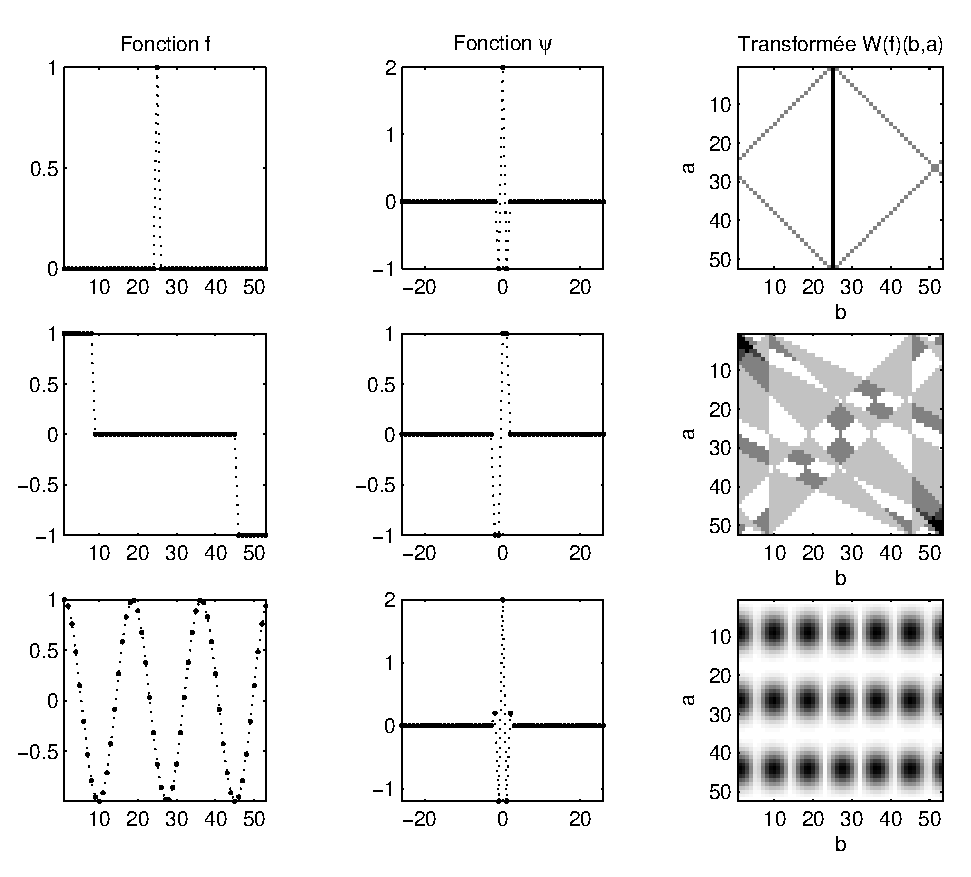
\includegraphics[scale=0.7]{images/ondelettes-corps-finis}
    \end{center}
    \caption{Wavelet transform on $ \FF_{53} $}
              \label{wavelets-finite-body}
\end{figure}
\end{exo}
 

